\begin{center}
\vfill
    \chapter{Meccanica quantistica}
    \label{blx:Quantistica\therefsection}
\vfill

\minitoc
\newpage
\end{center}
\justify

\section{Crisi della Fisica Classica e Nascita della Meccanica Quantistica}
\label{crisi-meccanica-quantistica}

All'inizio del Novecento, il modello matematico basato sulla fisica classica (Meccanica Newtoniana ed Elettrodinamica di Maxwell) si rivelò inadeguato a descrivere con successo numerosi fenomeni osservati su scala microscopica. Queste \textbf{incongruenze} tra teoria ed esperimento segnarono l'inizio di una profonda revisione dei fondamenti della fisica.

La fisica classica non era in grado di spiegare in modo soddisfacente i seguenti fenomeni, che richiedevano l'introduzione della \textbf{quantizzazione}:
\begin{itemize}
\item
    \textbf{La Stabilità dell'Atomo di Rutherford}: Secondo l'elettrodinamica classica, un elettrone in orbita attorno al nucleo (in moto accelerato) dovrebbe emettere continuamente radiazione elettromagnetica, perdendo energia e spiraleggiando verso il nucleo nel giro di una frazione di secondo. Al contrario, gli atomi sono \textbf{strutture stabili};
\item
    \textbf{La Distribuzione Spettrale della Radiazione del Corpo Nero}: La teoria classica (legge di Rayleigh-Jeans) prevedeva che l'energia emessa da un corpo nero divergesse alle alte frequenze, portando a una quantità di energia infinita (la cosiddetta \textbf{catastrofe ultravioletta} o \textbf{Rayleigh-Jeans catastrophe}), in netto contrasto con i dati sperimentali. Questo problema fu risolto da Planck (1900) postulando che l'energia fosse emessa in pacchetti discreti ($E=h\nu$);
\item
    \textbf{L'Effetto Fotoelettrico}: La luce incidente su una superficie metallica può liberare elettroni solo se la sua frequenza supera un valore soglia specifico, indipendentemente dall'intensità della luce stessa. La teoria ondulatoria classica non poteva spiegare questa dipendenza dalla frequenza. Il fenomeno fu spiegato da Einstein (1905) introducendo il concetto di \textbf{fotone} (quanto di luce).
\end{itemize}

Parallelamente o immediatamente dopo la risoluzione di questi problemi, una serie di esperimenti fornirono ulteriori e definitive prove a sostegno della necessità di una nuova teoria quantistica:

\begin{itemize}
\item
    \textbf{Spettri di Emissione e Assorbimento Atomico}: Gli atomi emettono o assorbono luce solo a \textbf{frequenze discrete} e ben definite, anziché su uno spettro continuo. Questo risultato fu la prova diretta che l'energia degli elettroni all'interno dell'atomo è \textbf{quantizzata} in livelli specifici (modello di Bohr, 1913);
\item
    \textbf{Esperimento di Stern-Gerlach (1922)}: Un fascio di atomi (come l'argento) fatto passare attraverso un campo magnetico non uniforme si divide in un numero finito e discreto di componenti (storicamente, due). Ciò dimostrò la \textbf{quantizzazione spaziale} del momento angolare e, successivamente, l'esistenza dello \textbf{spin} (momento angolare intrinseco) dell'elettrone, che non ha alcun analogo classico;
\item
    \textbf{Diffrazione di Elettroni e Doppio Slit (Davisson-Germer, 1927)}: L'osservazione che particelle come gli elettroni producano figure di interferenza tipiche delle onde confermò la \textbf{dualità onda-particella} proposta da De Broglie (1924), evidenziando che le particelle microscopiche si comportano come onde in determinate circostanze.
\end{itemize}

Queste difficoltà e scoperte portarono alla necessità di rivedere i fondamenti della fisica. Nacque così la \textbf{Meccanica Quantistica}, una nuova teoria che descrive il comportamento della materia e dell'energia su scala microscopica, introducendo concetti fondamentali come la \textbf{quantizzazione}, la \textbf{probabilità} e la \textbf{dualità onda-particella} \cite{messiah1961quantum, wichmann1971quantistica, feynman1965vol3}.

\subsection{Stabilità dell'Atomo e Collasso Elettronico (Critica al Modello di Rutherford)}\label{stabilituxe0-dellelettrone}

Il problema della stabilità atomica rappresenta una delle incongruenze più acute tra teoria classica e osservazione.
Secondo l'elettrodinamica classica, formalizzata dalle equazioni di Maxwell, una carica elettrica in \textbf{moto accelerato} (come l'elettrone in orbita attorno al nucleo nel modello planetario di Rutherford) dovrebbe emettere continuamente energia sotto forma di \textbf{radiazione elettromagnetica}. 

Questo rilascio continuo di energia implicherebbe una rapida \textbf{perdita di energia cinetica} da parte dell'elettrone e una conseguente riduzione del raggio orbitale, portando al \textbf{collasso} dell'elettrone sul nucleo in un tempo stimato di circa $10^{-11}$ secondi.

Tuttavia, l'evidenza sperimentale dimostra che gli atomi sono strutture intrinsecamente \textbf{stabili}, che esistono indefinitamente nel tempo senza collassare. Questa lampante discrepanza richiese l'abbandono dei principi classici per la descrizione della materia a livello microscopico.

La prima risoluzione teorica di questa crisi fu proposta da \textbf{Niels Bohr nel 1913}, attraverso l'introduzione di \textbf{postulati quantistici}: l'elettrone può occupare solo determinate \textbf{orbite stazionarie} (o stati quantici) in cui, per definizione, \textbf{non emette alcuna radiazione}. L'emissione o l'assorbimento di energia avviene solo durante la transizione tra questi livelli discreti, sotto forma di quanti di energia (fotoni), in accordo con la relazione di Planck ($E = h\nu$).

\subsection{Radiazione del Corpo Nero e la Quantizzazione di Planck}\label{corpo-nero}

Il \textbf{corpo nero} è un oggetto ideale che assorbe completamente tutta la radiazione elettromagnetica incidente, senza rifletterla né trasmetterla. Di conseguenza, per la conservazione dell'energia, quando riscaldato, emette radiazione termica a ogni lunghezza d'onda, e la distribuzione di questa energia è funzione esclusiva della sua temperatura.

Sebbene il corpo nero sia un'astrazione teorica, può essere approssimato sperimentalmente da una cavità con pareti interne nere e una piccola apertura. La radiazione che entra ha una probabilità estremamente bassa di uscire, simulando il comportamento ideale.

\begin{figure}[ht]
\centering
\resizebox{0.5\textwidth}{!}{%
\begin{tikzpicture}[scale=1.3]

  \shade[top color=black!60,bottom color=black!80,shading angle=10] % background
    (7:1) arc (7:355:1);
  
  \fill[thick,black,postaction=decorate, % rough inner surface
    decoration={markings,mark=between positions 0.55 and 1 step 0.03 with {
                  \node[transform shape,inner sep=1pt]
                  (hit\pgfkeysvalueof{/pgf/decoration/mark info/sequence number}) {};
    }}]
    (7:1) arc (7:353:1) --++ (-7:-0.18)
    decorate[decoration={random steps,segment length=2,amplitude=1pt}]
        {arc (-7:-353:0.82)} -- cycle;

% Raggi che entrano e colpiscono la circonferenza
\draw[red,thick,->] (2.3,0) -- (0.9,0); % ingresso
\draw[red,thick,->] (0.9,0) -- (-0.1,-0.8); % primo rimbalzo
\draw[red,thick,->] (-0.1,-0.8) -- (0.6,0.5); % secondo rimbalzo
\draw[red,thick,->] (0.6,0.5) -- (-0.8,-0.1); % terzo rimbalzo
\draw[red,thick,->] (-0.8,-0.1) -- (-0.2,-0.51); % quarto rimbalzo

% Etichetta raggio
\node[red] at (3.5,0) {Raggio incidente};

\end{tikzpicture}
}
\caption{Modello pratico di corpo nero, come una cavità con una piccola apertura}
\label{fig:4_CorpoNero}
\end{figure}


Secondo la fisica classica, in particolare la teoria basata sulla legge di \textbf{Rayleigh-Jeans}, l'intensità della radiazione emessa per unità di frequenza ($I(\nu, T)$) dovrebbe aumentare indefinitamente con l'aumento della frequenza ($\nu$). Questa previsione teorica, che prevedeva una divergenza dell'energia alle alte frequenze, è nota come \textbf{catastrofe ultravioletta} e contraddiceva clamorosamente i risultati sperimentali.

\begin{figure}[ht]
\centering
\resizebox{0.5\textwidth}{!}{%

% BLACK BODY - 3000, 4000, 5000K, Wien's displacement law
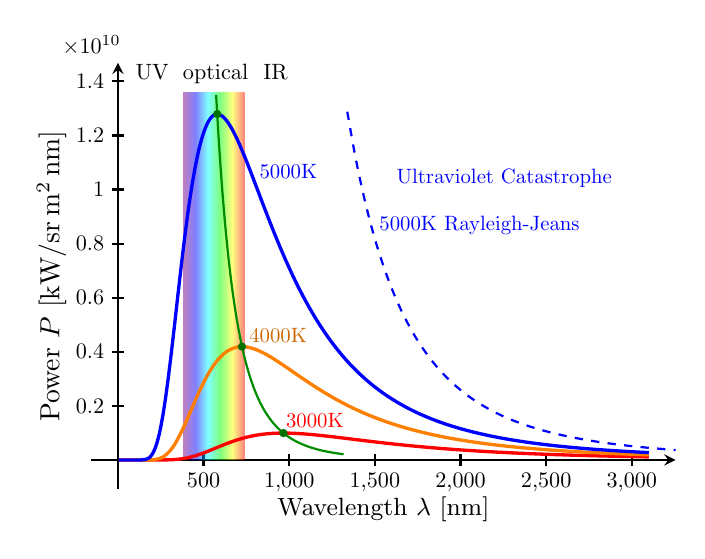
\begin{tikzpicture}
% redraw axis on top
\makeatletter \newcommand{\pgfplotsdrawaxis}{\pgfplots@draw@axis} \makeatother
\pgfplotsset{axis line on top/.style={after end axis/.append code={\pgfplotsdrawaxis}}
}

% CUSTOM COLORS
% See https://tikz.net/blackbody_color/
\definecolor{1000K}{rgb}{1,0.0337,0}
\definecolor{2000K}{rgb}{1,0.2647,0.0033}
\definecolor{3000K}{rgb}{1,0.4870,0.1411}
\definecolor{4000K}{rgb}{1,0.6636,0.3583}
\definecolor{5000K}{rgb}{1,0.7992,0.6045}
\definecolor{6000K}{rgb}{1,0.9019,0.8473}
\definecolor{8000K}{rgb}{0.7874,0.8187,1}
\definecolor{10000K}{rgb}{0.6268,0.7039,1}
\pgfdeclareverticalshading{rainbow}{100bp}{
  color(0bp)=(red); color(25bp)=(red); color(35bp)=(yellow);
  color(45bp)=(green); color(55bp)=(cyan); color(65bp)=(blue);
  color(75bp)=(violet); color(100bp)=(violet)
}
\colorlet{myred}{red!70!black}
\colorlet{mygreen}{green!70!black}
\colorlet{mydarkgreen}{green!55!black}

% PLANCK & RAYLEIGH-JEANS
% 2hc^2/lambda^5 = 2 * 6.62607015e-34 * 299792458^2
%                = 1.191042972e-16
%    W.m -> kW.nm: 1.191042972e26
%  hc/k lambda T = 6.62607015e-34*299792458/(1.38064852e-23)
%                = 0.01438777378
%         m -> nm: 0.01438777378e9
% 2ckT/lambda^4  = 2 * 299792458 * 1.38064852e-23
%                = 8.278160269e-15
%    W.m -> kW.nm: 8.278160269e18
\pgfmathdeclarefunction{planck}{2}{%
  \pgfmathparse{1.191042972e26/(#1^5)/(exp(0.01439e9/(#1*#2))-1)}%
}
\pgfmathdeclarefunction{rayleighjeans}{2}{%
  \pgfmathparse{8.278160269e18*#2/(#1^4)}%
}
\pgfmathdeclarefunction{wien}{2}{%
  \pgfmathparse{1.191042972e26/(#1^5)*exp(-0.01439e9/(#1*#2))}%
}
\pgfmathdeclarefunction{lampeak}{1}{% % Wien's displacement law
  \pgfmathparse{2.898e6/#1}%
}
  \message{^^JBlack body, Wien's displacement law}
  \def\N{60}
  \def\xmax{3100}
  \def\ymax{1.36e10}
  \def\tick#1#2{\draw[thick] (#1+.01*\ymax) -- (#1-.01*\ymax) node[below=-.5pt,scale=0.75] {#2};}
  \begin{axis}[
      every axis plot/.style={
        very thick,mark=none,samples=\N,domain=5:\xmax,smooth},
      xmin=(-.05*\xmax), xmax=(1.05*\xmax),
      ymin=(-.08*\ymax), ymax=(1.08*\ymax),
      restrict y to domain=0:\ymax,
      axis lines=middle,
      axis line style=thick,
      %enlargelimits=upper, % extend the axes a bit to the right and top
      tick style={black,thick},
      ticklabel style={scale=0.8},
      %xtick style={draw=none},xticklabels=none,
      max space between ticks=26,
      xlabel={Wavelength $\lambda$ [nm]},
      ylabel={Power $P$ [kW/sr\,m$^2$\,nm]},
      xlabel style={at={(rel axis cs:0.5,0)},below=-1pt,font=\small},
      ylabel style={at={(rel axis cs:-0.11,0.5)},rotate=90},
      width=9cm, height=7cm,
      %clip=false
      tick scale binop=\times,
      every y tick scale label/.style={at={(rel axis cs:0,1)},anchor=south}]
    ]
    
    % RAINBOW
    \shade[shading=rainbow,shading angle=90,opacity=0.5] (380,0) rectangle (740,\ymax);
    \node[above=-1pt,scale=0.8] at (200,\ymax) {\strut UV}; % 10 - 400 nm
    \node[above=-1pt,scale=0.8] at (570,\ymax) {\strut optical}; % 380 - 740 nm
    \node[above=-1pt,scale=0.8] at (920,\ymax) {\strut IR}; % 740 - 1050 nm
    
    % PLANCK
    \addplot[red]    {planck(x,3000)};
    \addplot[orange] {planck(x,4000)};
    \addplot[blue,samples=3*\N] {planck(x,5000)};
    \addplot[dashed,thick,blue,domain=1000:3500] {rayleighjeans(x,5000)};
    
    % MAXIMUM (Wien's displacement law)
    \addplot[mydarkgreen,thick,variable=T,domain=2200:4000,samples=40]
      ({lampeak(T)},{planck(lampeak(T),T)});
    \addplot[mydarkgreen,thick,variable=T,domain=4000:5200,samples=100]
      ({lampeak(T)},{planck(lampeak(T),T)});
    \fill[mydarkgreen!80!black] ({lampeak(3000)},{planck(lampeak(3000),3000)}) circle(1.5pt);
    \fill[mydarkgreen!80!black] ({lampeak(4000)},{planck(lampeak(4000),4000)}) circle(1.5pt);
    \fill[mydarkgreen!80!black] ({lampeak(5000)},{planck(lampeak(5000),5000)}) circle(1.5pt);
    
    % LABELS
    \node[above=0pt,scale=0.75,red] at (1150,{planck(1150,3000)}) {\SI{3000}{K}};
    \node[above right=-1pt,scale=0.75,orange!80!black] at (740,{planck(740,4000)}) {\SI{4000}{K}};
    \node[above right=-1pt,scale=0.75,blue] at (800,{planck(800,5000)}) {\SI{5000}{K}};
    \node[above right=-1pt,scale=0.75,blue] at (1500,{rayleighjeans(1500,5000)}) {\SI{5000}{K} Rayleigh-Jeans};
    \node[above right=-1pt,scale=0.75,blue] at (1600,{rayleighjeans(1430,5000)}) {Ultraviolet Catastrophe};
    
  \end{axis}
\end{tikzpicture}

}
\caption{Confronto tra la previsione classica (Rayleigh-Jeans) e i dati sperimentali che mostrano la catastrofe ultravioletta}
\label{fig:4_CatastrofeUV}
\end{figure}

In realtà, lo spettro di emissione del corpo nero dipende strettamente dalla temperatura, presentando un andamento continuo e finito: l'intensità raggiunge un massimo a una specifica lunghezza d'onda, che si sposta verso valori più corti all'aumentare della temperatura (Legge dello spostamento di Wien), per poi decrescere.

La risoluzione teorica di questo problema fondamentale fu proposta da \textbf{Max Planck nel 1900}, segnando la nascita della meccanica quantistica. Planck ipotizzò che l'energia scambiata tra gli oscillatori atomici delle pareti della cavità e la radiazione non fosse continua, ma avvenisse in pacchetti discreti o \textit{quanti} di energia.

L'energia emessa o assorbita è quindi un multiplo intero ($n$) di una quantità elementare, proporzionale alla frequenza ($\nu$) della radiazione:

\[
E = h\nu
\]

dove $E$ è l'energia del quanto (per $n=1$), $\nu$ è la frequenza della radiazione, e $h$ è la \textbf{costante di Planck}. Questa ipotesi permise a Planck di derivare una formula che descriveva correttamente l'intero spettro osservato.

\subsection{Effetto fotoelettrico}\label{effetto-fotoelettrico}

L'effetto fotoelettrico è un fenomeno di interazione tra la radiazione elettromagnetica e la materia, caratterizzato dall'emissione di elettroni (detti \textbf{fotoelettroni}) da una superficie, generalmente metallica, quando irradiata da energia elettromagnetica. 

Sperimentalmente, l'effetto si osserva ponendo due elettrodi metallici all'interno di un'ampolla sotto vuoto spinto. Quando l'elettrodo (catodo) viene irradiato, gli elettroni espulsi generano una \textbf{corrente elettrica} rilevabile sull'elettrodo opposto (anodo).

\begin{figure}[ht]
\centering
\includegraphics[width=2.98611in,height=2.19407in,alt={P1636\#yIS1}]{media/4_Quantiatica/image33.pdf}\caption{Circuito per l'effetto fotoelettrico}
\end{figure}

Gli elettroni emessi dall'elettrodo irradiato, dotati di energia cinetica non nulla, vengono accelerati dal campo elettrico generato da una batteria, raggiungendo il secondo elettrodo collegato al polo positivo. In questo modo, si chiude il circuito elettrico e si rileva una corrente.

L'energia cinetica massima ($K_{\max}$) dei fotoelettroni può essere misurata applicando una \textbf{tensione di arresto} ($V_s$): una differenza di potenziale opposta e sufficiente ad annullare la corrente, impedendo anche agli elettroni più energetici di raggiungere l'anodo. L'energia cinetica massima è quindi data da $K_{\max} = e V_s$.

Si applica una differenza di potenziale tale da bloccare la circolazione di corrente nel circuito, nonostante l'irraggiamento dell'elettrodo. In questa situazione, un elettrone, espulso per effetto fotoelettrico con una certa energia cinetica, si trova in un campo elettrico che lo decelera fino a farlo tornare sull'elettrodo che l'ha prodotto. Nota la tensione applicata, si riesce a determinare l'energia dell'elettrone espulso.

Secondo la teoria ondulatoria classica, l'energia trasferita agli elettroni e, di conseguenza, la loro energia cinetica massima ($K_{\max}$), avrebbe dovuto:
\begin{enumerate}
    \item Dipendere dall'\textbf{intensità} della radiazione (una luce più brillante avrebbe dovuto liberare elettroni più energetici).
    \item Manifestarsi dopo un certo \textbf{ritardo temporale} per accumulare l'energia necessaria.
\end{enumerate}
L'esperimento smentì entrambe le previsioni: l'emissione è \textbf{istantanea} e $K_{\max}$ dipende esclusivamente dalla \textbf{frequenza} ($\nu$) della radiazione incidente, e non dalla sua intensità. Inoltre, esiste una \textbf{frequenza di soglia} ($\nu_0$) al di sotto della quale l'emissione non avviene affatto, anche ad alta intensità.


Albert Einstein risolse questa incongruenza nel 1905, estendendo l'ipotesi di Planck: la luce non si comporta solo come un'onda, ma è composta da particelle discrete, i \textbf{fotoni} (quanti di luce), ciascuno con energia:

\[
E = h\nu
\]

dove $h$ è la costante di Planck e $\nu$ è la frequenza. L'emissione di un elettrone avviene in un processo di interazione \textbf{uno-a-uno} tra un singolo fotone e un singolo elettrone.

L'equazione fondamentale che descrive l'effetto fotoelettrico è:

$$K_{\max} = E - \phi = h\nu - \phi$$

dove $K_{\max}$ è l'energia cinetica massima dell'elettrone espulso, $h\nu$ è l'energia del fotone incidente, e $\mathbf{\phi}$ (o $W_0$) è la \textbf{funzione lavoro} (l'energia minima necessaria per estrarre l'elettrone dalla superficie metallica).

Questa spiegazione, che attribuiva alla luce una \textbf{natura corpuscolare} (dualità onda-particella), valse ad Einstein il Premio Nobel per la Fisica nel 1921.

\subsection{L'Esperimento della Doppia Fenditura e la Dualità Onda-Particella}\label{double-slit}

Mentre la crisi della fisica classica era iniziata con la natura quantizzata della luce (fotoni, 1905), l'esperimento della \textbf{doppia fenditura} (o \textbf{double slit}) ha esteso il dualismo alla \textbf{materia}, rivelando la natura ondulatoria di particelle come gli elettroni. Questo risultato ha messo definitivamente in crisi la visione strettamente corpuscolare della materia.

Nell'esperimento cruciale, un fascio di elettroni (o altre particelle) viene inviato contro una parete dotata di due fenditure parallele. Sullo schermo di rilevazione posto dietro le fenditure, anziché osservare le due bande nette previste per le particelle classiche, si forma una \textbf{figura di interferenza}: una sequenza di frange chiare (interferenza costruttiva) e scure (interferenza distruttiva), un comportamento tipico ed esclusivo dei fenomeni ondulatori.

\begin{figure}[ht]
\centering
\includegraphics[width=3.02778in,height=2.29079in,alt={P1647\#yIS1}]{media/4_Quantiatica/image34.pdf}\caption{Figura di interferenza della doppia fenditura}
\end{figure}

Il comportamento degli elettroni in questo esperimento può essere interpretato attraverso il principio di Huygens dei fenomeni ondulatori, secondo cui ogni punto \(d\Sigma\) di un fronte d'onda \(\Sigma\) può essere considerato come sorgente secondaria di onde sferiche. La perturbazione risultante in un punto dello spazio è data dalla sovrapposizione di tutte le onde secondarie che vi giungono.

Il risultato è sorprendente perché, anche inviando gli elettroni \textbf{uno alla volta}, il pattern di interferenza si accumula gradualmente, suggerendo che ogni particella interferisca in qualche modo \textbf{con sé stessa}.

Gli elettroni sono particelle dotate di massa, infatti, in altri esperimenti, come l'effetto fotoelettrici, gli elettroni interagiscono con i fotoni come particelle, attraverso urti elastici. Questi due comportamenti apparentemente contraddittori (particella in urti elastici come nell'effetto fotoelettrico; onda nella doppia fenditura) hanno portato alla formulazione del concetto di \textbf{dualismo onda-corpuscolo}.

Nel 1924, \textbf{Louis de Broglie} propose l'ipotesi che a ogni particella materiale, con quantità di moto $p$, fosse associata un'onda, definita \textbf{onda di materia}, la cui lunghezza d'onda ($\lambda$) è inversamente proporzionale alla quantità di moto stessa:

\[
\lambda = \dfrac{h}{p}
\]

dove $h$ è la costante di Planck. Questa ipotesi teorica fu confermata sperimentalmente nel 1927 dagli esperimenti di \textbf{Davisson e Germer} e da \textbf{G.P. Thomson} sulla diffrazione di elettroni, che rappresenta uno dei pilastri fondamentali della meccanica quantistica.

\subsection{Esperimento di Stern e Gerlach: La Quantizzazione dello Spin}\label{esperimento-di-stern-e-gerlach}

L'esperimento di Stern e Gerlach, condotto nel 1922, ha fornito una delle prove sperimentali più dirette e convincenti della \textbf{quantizzazione del momento angolare} e ha rivelato l'esistenza di una proprietà intrinseca delle particelle: lo \textbf{spin}.

Nel setup sperimentale, un fascio di atomi d'argento (il cui momento angolare deriva quasi interamente dall'unico elettrone nel guscio esterno) viene fatto passare attraverso un \textbf{campo magnetico fortemente non uniforme}. 

Secondo la fisica classica, il momento magnetico degli atomi, orientandosi in modo continuo rispetto al campo, avrebbe dovuto produrre un'unica linea o una \textbf{distribuzione continua} sullo schermo di rilevazione.

Tuttavia, ciò che si osserva è una \textbf{separazione netta} del fascio in \textbf{due sole componenti distinte}. Questo risultato indica inequivocabilmente che il momento magnetico degli atomi, e quindi il loro momento angolare totale $L$, non può assumere valori arbitrari (come previsto dalla classica), ma solo un insieme finito e discreto di orientamenti spaziali.

In particolare, per gli atomi d'argento, la separazione in due componenti dimostra la quantizzazione dello \textbf{spin} dell'elettrone, per cui la sua proiezione lungo la direzione del campo può assumere solo due valori: $m_s = +1/2$ (spin "su") e $m_s = -1/2$ (spin "giù").

Questo esperimento ha dimostrato che:

\begin{itemize}
\item Il momento angolare (e il momento magnetico associato) è \textbf{quantizzato} spazialmente (quantizzazione spaziale).
\item Lo \textbf{spin} è una proprietà quantistica intrinseca e fondamentale delle particelle subatomiche, priva di analogo classico.
\item Le misure di grandezze quantistiche non danno risultati continui, ma solo \textbf{valori discreti} (autovalori), confermando il carattere non deterministico e non continuo della realtà microscopica.
\end{itemize}

L'esperimento di Stern-Gerlach è un pilastro della meccanica quantistica, poiché mostra in modo diretto la discrezione degli stati quantici.

\subsection{Spettri di Assorbimento e di Emissione: Evidenza della Quantizzazione Atomica}\label{spettro-di-assorbimento}

Lo \textbf{spettro di assorbimento} di un elemento chimico è l'insieme delle radiazioni elettromagnetiche assorbite quando la sostanza viene esposta a una sorgente luminosa a spettro continuo. Le sostanze assorbono energia solamente a determinate frequenze specifiche, dando origine a uno \textbf{spettro a righe scure} caratteristico.

Nei primi anni del Novecento, l'incapacità della meccanica classica di prevedere questi spettri a righe rappresentava un'ulteriore prova della sua inadeguatezza. Secondo la fisica classica, un atomo dovrebbe assorbire o emettere radiazioni su tutte le frequenze. Invece, l'osservazione che l'assorbimento avvenisse solo a frequenze discrete, indipendentemente dall'intensità, suggeriva l'esistenza di un meccanismo interno \textbf{quantizzato}.

Lo spettro risultante, osservato a valle dell'esposizione, è dato dalla radiazione incidente privata delle lunghezze d'onda assorbite dal materiale. In altre parole, lo spettro presenta delle bande scure, corrispondenti alle frequenze assorbite.

\begin{figure}[ht]
\centering
\includegraphics[width=3.34722in,height=2.81542in,alt={P1658\#yIS1}]{media/4_Quantiatica/image35.pdf}\caption{Spettro di assorbimento e di emissione}
\end{figure}

Già prima della formulazione teorica, la regolarità degli spettri atomici fu descritta empiricamente. In particolare, per l'atomo di idrogeno, \textbf{Johannes Rydberg} propose una formula per calcolare le lunghezze d'onda delle righe spettrali (sia di assorbimento che di emissione):

\[
\dfrac{1}{\lambda} = R_{H}\left( \dfrac{1}{n_{1}^{2}} - \dfrac{1}{n_{2}^{2}} \right)
\]

dove $R_H$ è la costante di Rydberg e $n_1, n_2$ sono \textbf{numeri interi positivi} ($n_1, n_2 \in \mathbb{N}$, con $n_2 > n_1$). La dipendenza da numeri interi era un indizio potentissimo dell'esistenza di \textbf{livelli energetici discreti} all'interno dell'atomo.

Sebbene la formula di Rydberg fosse predittiva, non ne spiegava il fondamento fisico. La spiegazione teorica arrivò nel 1913 con il \textbf{modello atomico di Bohr}. Bohr postulò che:

\begin{itemize}
    \item L'energia dell'elettrone è \textbf{quantizzata} e confinata in livelli specifici ($E_n$);
    \item L'assorbimento (o l'emissione) di radiazione avviene solo quando l'elettrone compie una \textbf{transizione quantica} tra due di questi livelli discreti, con la frequenza del fotone emesso/assorbito data dalla differenza di energia tra i livelli: $\nu = (E_2 - E_1)/h$.
\end{itemize}

Il modello di Bohr fornì la prima giustificazione fisica della formula di Rydberg, legando i numeri interi $n_1$ e $n_2$ ai numeri quantici dei livelli energetici stazionari dell'atomo.

\section{Teoria della meccanica quantistica}\label{teoria-della-meccanica-quantistica}

La Meccanica Quantistica (MQ) costituisce il quadro teorico fondamentale per la descrizione del comportamento della materia e dell'energia su scala microscopica. In fisica teorica, la MQ viene sviluppata attraverso due principali formulazioni:

\begin{itemize}
    \item La MQ \textbf{non relativistica}: sufficiente per descrivere la struttura degli atomi, le molecole e la dinamica delle particelle che si muovono a velocità ben inferiori a quella della luce ($v \ll c$). Questa modellazione si basa sull'equazione di Schrödinger.
    \item La MQ \textbf{relativistica}: necessaria per trattare particelle che si muovono a velocità prossime a $c$ e per le interazioni ad alta energia, un campo noto come \textbf{Teoria Quantistica dei Campi} (QFT).
\end{itemize}

La teoria quantistica relativistica più celebre e di successo è l'\textbf{Elettrodinamica Quantistica} (QED, \textit{Quantum Electrodynamics}). Essa descrive con straordinaria precisione le interazioni elettromagnetiche, modellando il comportamento dei fotoni (mediatori del campo) e le loro interazioni con le particelle cariche, come gli elettroni. 

\begin{figure}[h!]
    \centering
    \resizebox{1\textwidth}{!}{
        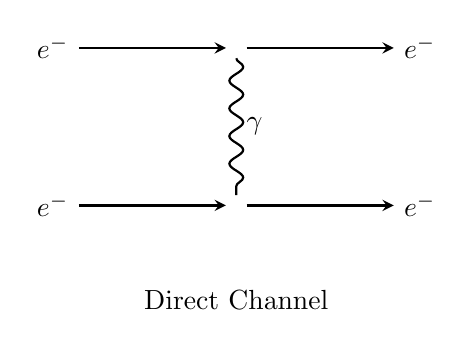
\begin{tikzpicture}[>=stealth, thick]

%--- Direct Channel ---
% Fermions in ingresso
\node[left] (a1) at (-2,1) {$e^-$};
\node[left] (a2) at (-2,-1) {$e^-$};

% Fermions in uscita
\node[right] (b1) at (2,1) {$e^-$};
\node[right] (b2) at (2,-1) {$e^-$};

% Vertici
\node (v1) at (0,1) {};
\node (v2) at (0,-1) {};

% Linee fermioniche
\draw[->] (a1) -- (v1);
\draw[->] (a2) -- (v2);
\draw[->] (v1) -- (b1);
\draw[->] (v2) -- (b2);

% Fotone
\draw[decorate, decoration={snake}] (v1) -- node[right] {$\gamma$} (v2);

% Titolo
\node at (0,-2.2) {Direct Channel};

\end{tikzpicture}
\hspace{2cm}
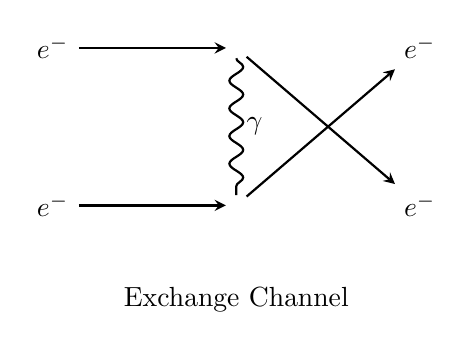
\begin{tikzpicture}[>=stealth, thick]

%--- Exchange Channel ---
% Fermions in ingresso
\node[left] (c1) at (-2,1) {$e^-$};
\node[left] (c2) at (-2,-1) {$e^-$};

% Fermions in uscita
\node[right] (d1) at (2,1) {$e^-$};
\node[right] (d2) at (2,-1) {$e^-$};

% Vertici
\node (v3) at (0,1) {};
\node (v4) at (0,-1) {};

% Linee fermioniche con scambio
\draw[->] (c1) -- (v3);
\draw[->] (c2) -- (v4);
\draw[->] (v3) -- (d2);
\draw[->] (v4) -- (d1);

% Fotone
\draw[decorate, decoration={snake}] (v3) -- node[right] {$\gamma$} (v4);

% Titolo
\node at (0,-2.2) {Exchange Channel};

\end{tikzpicture}

    }
    \caption{Diagrammi di Feynman per lo scattering elettrone-elettrone (Møller). Il diagramma a sinistra rappresenta il canale diretto, e il diagramma a destra rappresenta il canale di scambio.}
    \label{fig:electron_electron_scattering_arranged}
\end{figure}

Una delle previsioni cruciali della formulazione relativistica della MQ (in particolare, l'equazione di Dirac del 1928, fondamento della QED) è l'esistenza delle \textbf{antiparticelle}, entità con carica e numeri quantici opposti rispetto alla materia ordinaria. Un esempio è il \textbf{positrone} ($e^{+}$), l'antiparticella dell'elettrone, scoperto sperimentalmente nel 1932.

La Meccanica Quantistica non relativistica si è sviluppata a partire dai contributi pionieristici di:
\begin{itemize}
    \item \textbf{Max Planck} (1900): con l'ipotesi della quantizzazione dell'energia ($E=h\nu$) per spiegare la radiazione del corpo nero.
    \item \textbf{Albert Einstein} (1905): con l'interpretazione quantistica dell'effetto fotoelettrico, introducendo il concetto di fotone.
    \item \textbf{Louis de Broglie} (1924): con la proposta della dualità onda-corpuscolo per la materia.
\end{itemize}

Questi contributi hanno posto le basi per la formulazione moderna della MQ, una teoria che abbandona il determinismo classico per descrivere il comportamento delle particelle microscopiche in termini \textbf{probabilistici}, introducendo concetti come la \textbf{funzione d’onda} ($\Psi$), il \textbf{principio di indeterminazione} (Heisenberg) e la \textbf{quantizzazione degli stati energetici} \cite{dirac1930principles, messiah1961quantum, wichmann1971quantistica, feynman1965vol3, landau1975quantistica_rel}.

\subsection{Quantizzazione della materia}\label{quantizzazione-della-materia}

L'ipotesi fondamentale della meccanica quantistica è che le grandezze fisiche a livello microscopico siano \textbf{quantizzate}: esse non variano in modo continuo, ma possono assumere solo \textbf{valori discreti} (autovalori), spesso multipli interi di una quantità fondamentale. Questo principio, inizialmente suggerito da Planck per l'energia della radiazione e da Einstein per il fotone, è cruciale per descrivere la struttura della materia.

Gli elettroni all'interno di un atomo occupano \textbf{livelli energetici stazionari} ($E_1, E_2, \ldots$) che rappresentano stati quantici definiti. Poiché gli elettroni possono occupare solo questi livelli quantizzati, non sono soggetti al collasso sul nucleo (come previsto dalla fisica classica), garantendo la \textbf{stabilità dell'atomo}.

Un fotone incidente sull'atomo può essere assorbito dall'elettrone solo se la sua energia è \textbf{esattamente uguale} alla differenza di energia tra due livelli ammissibili ($E_f$ e $E_i$):

\[
E_{\text{fotone}} = E_f - E_i
\]

L'energia del fotone è data dalla relazione di Planck:

\[
E = h\nu
\]

dove $E$ è l'energia del fotone, $\nu$ è la sua frequenza, e $h$ è la costante di Planck. Da questa condizione deriva il fenomeno degli \textbf{spettri a righe}: l'atomo assorbe o emette radiazione solo alle frequenze $\nu$ ben definite, come dimostrato dalla formula empirica di Rydberg.

Se il fotone viene assorbito, l'elettrone subisce una transizione (eccitazione) a un livello energetico superiore ($E_f$). Successivamente, l'elettrone può ritornare a un livello inferiore (rilassamento), emettendo un fotone con un'energia pari alla differenza energetica tra i due stati.

\subsection{Dualismo Onda-Particella (Ipotesi di De Broglie)}\label{dualismo-onda-particella} 
 
L'ipotesi di \textbf{Louis de Broglie}, formulata nel 1924, ha esteso il dualismo onda-corpuscolo (già riconosciuto per la luce) alla \textbf{materia}. Secondo questa ipotesi, a ogni particella materiale, come l'elettrone, è associata un'onda (l'\textbf{onda di materia}), descritta da una \textbf{funzione d'onda} $\Psi(\vec{r}, t)$, che racchiude le informazioni sullo stato quantico della particella. 
 
Le relazioni di De Broglie stabiliscono il legame quantitativo tra le proprietà corpuscolari (Energia $E$, Quantità di moto $p$) e le proprietà ondulatorie (Frequenza $\nu$, Lunghezza d'onda $\lambda$). 
 
L'energia ($E$) della particella è legata alla frequenza ($\nu$) e alla pulsazione ($\omega$) dell'onda associata dalla relazione di Planck: 

\[
E = h\nu
\]

dove \(E\) è l'energia associata all'onda, \(\nu\) è la frequenza, e \(h\) è la costante di Planck. La pulsazione è legata alla frequenza da:

\[
\omega = 2\pi\nu
\]

Sostituendo nella formula dell'energia, si ottiene:

\[
E = \dfrac{h}{2\pi}\omega = \hslash\omega
\]

dove:

\[
\hslash = \dfrac{h}{2\pi}
\]

è la \textbf{costante di Planck ridotta}. 

Alla particella è anche associata una quantità di moto \(p\). Per l'ipotesi di de Broglie, la quantità di moto ($p$) è legata al \textbf{numero d'onda} ($k$) e alla lunghezza d'onda ($\lambda$): 

\[
p = \hslash k
\]

dove \(k\) è il \textbf{numero d'onda} definito come:

\[
k = \dfrac{2\pi}{\lambda}
\]

Sostituendo la definizione di $\hslash$ e $k$, si ottiene la relazione fondamentale che quantifica il dualismo:

\[
\lambda = \dfrac{h}{p}
\]

Questa formula dimostra che maggiore è la quantità di moto della particella, minore è la lunghezza d'onda associata, spiegando perché gli effetti ondulatori non siano osservabili su scala macroscopica. 
 
Mentre le relazioni di De Broglie si applicano a tutte le particelle, il loro contesto energetico è definito dalla relatività. Per una particella con massa a riposo $m_0$, la relazione completa tra energia e quantità di moto è: 

\[
E^2 = (pc)^2 + (m_0c^2)^2
\]

In \textbf{regime non relativistico} ($v \ll c$), l'energia cinetica domina, e la relazione $\lambda = h/p$ è l'approssimazione valida. Il \textbf{fotone} ($m_0=0$) rappresenta il limite estremo, dove la relazione $p = h/\lambda$ è ottenuta direttamente dalle leggi dell'elettromagnetismo e di Planck ($p = E/c = h\nu/c$). 
 
Queste relazioni confermano in modo definitivo il \textbf{dualismo onda-corpuscolo} alla base della meccanica quantistica. 

\subsection{Funzione d'onda associata alla particella}\label{funzione-donda-associata-alla-particella}

L'ipotesi di de Broglie stabilisce che a ogni particella (elettrone, protone, ecc.) è associata una \textbf{funzione d'onda} $\Psi(\vec{r}, t)$, che ne descrive lo stato quantico. Nel caso più semplice di una \textbf{particella libera} in moto (ad esempio, lungo l'asse $x$), la funzione d'onda assume la forma di un'onda piana, espressa mediante un esponenziale complesso:

\[
\Psi(x,t) = A \exp\left( j(kx - \omega t) \right)
\]

dove $A$ è l'ampiezza dell'onda, \(k\) è il numero d'onda, \(\omega\) è la pulsazione, e \(j\) è l'unità immaginaria (\(j^2 = -1\)). Una qualsiasi forma d'onda può essere ottenuta come sovrapposizione di infinite onde piane.

I parametri \(k\) (numero d'onda) e \(\omega\) (pulsazione) possono essere espressi in funzione delle grandezze fisiche della particella:

\[
k = \dfrac{p}{\hslash} \quad \text{e} \quad \omega = \dfrac{E}{\hslash}
\]

Sostituendo i parametri ondulatori ($k$ e $\omega$) con le grandezze fisiche della particella (quantità di moto $p$ ed Energia $E$) tramite la relazione di De Broglie ($k = p/\hslash$ e $\omega = E/\hslash$), si ottiene:

\[
\Psi(x,t) = A \exp\left( \dfrac{j}{\hslash}\left(px - Et\right) \right)
\]

Nel caso tridimensionale, l'espressione è generalizzata utilizzando il prodotto scalare tra il vettore quantità di moto $\vec{p}$ e il vettore posizione $\vec{r}$:

\[
\Psi(\vec{r},t) = A \exp\left( \dfrac{j}{\hslash} \left(\vec{p} \cdot \vec{r} - Et\right) \right)
\]

Secondo l'\textbf{interpretazione di Born}, la funzione d'onda $\Psi(\vec{r}, t)$ non ha un significato fisico diretto, ma il suo modulo quadro, $|\Psi(\vec{r}, t)|^2$, rappresenta la \textbf{densità di probabilità} $P(\vec{r}, t)$ di trovare la particella nella posizione $\vec{r}$ al tempo $t$:

\[
P(\vec{r},t) = \left| \Psi(\vec{r},t) \right|^{2}
\]

Nel caso specifico dell'onda piana, la probabilità risulta uniforme in tutto lo spazio ($|\Psi|^2 = |A|^2 = \text{costante}$). Tuttavia, tale funzione si estende all'infinito e non è normalizzabile, pertanto non rappresenta una situazione fisica realistica di una particella localizzata. Per descrivere particelle localizzate, si utilizza il concetto di \textbf{pacchetti d’onda}, ottenuti come sovrapposizione di infinite onde piane con diverse lunghezze d'onda (e quindi diverse quantità di moto).

In questo contesto probabilistico, il concetto classico di orbita (inteso come traiettoria deterministica) non è più applicabile. La regione dello spazio in cui la probabilità di trovare l'elettrone è massima viene definita \textbf{orbitale} (per gli stati legati negli atomi).

\section{Principio di indeterminazione di Heisenberg}\label{principio-di-indeterminazione-di-heisenberg}

Il principio di indeterminazione di Heisenberg è coerente con l’interpretazione probabilistica della meccanica quantistica proposta da Born. Secondo questo principio, non è possibile conoscere con precisione e simultaneamente la posizione e la quantità di moto di una particella. Indicando con \({\Delta}x\) l’incertezza sulla posizione e con \({\Delta}p\) quella sulla quantità di moto, si ha:

\[
{\Delta}x {\Delta}p \geq \dfrac{\hslash}{2}
\]

Questo significa che, se la posizione viene determinata con estrema precisione (\({\Delta}x \rightarrow 0\)), l’incertezza sulla quantità di moto deve aumentare (\({\Delta}p \rightarrow \infty\)) per mantenere valida la disuguaglianza. Analogamente, maggiore è la precisione sulla misura della quantità di moto meno precisa è la conoscenza della posizione, ovvero \({\Delta}p \rightarrow 0\) allora \({\Delta}x \rightarrow \infty\).

Il principio può essere esteso anche alla coppia energia-tempo, come:

\[
{\Delta}E {\Delta}t \geq \dfrac{\hslash}{2}
\]

In questo contesto, $\Delta t$ rappresenta l'intervallo di tempo durante il quale l'energia del sistema è definita. Questo significa che una misura precisa dell’energia ($\Delta E \rightarrow 0$) richiede un intervallo di tempo $\Delta t$ sufficientemente lungo (tendente a infinito), mentre una misura molto rapida ($\Delta t$ piccolo) comporta una maggiore incertezza sull’energia ($\Delta E$ grande).

Questo principio rappresenta un limite fondamentale alla conoscenza dello stato di una particella e riflette la natura intrinsecamente probabilistica della meccanica quantistica.

L’indeterminazione può essere interpretata come una conseguenza del processo di misura. Per determinare la posizione di una particella, ad esempio un elettrone, è necessario interagire con essa, ad esempio mediante fotoni. Questa interazione modifica inevitabilmente lo stato della particella. Nel mondo macroscopico, tale effetto è trascurabile, poiché l’energia dei fotoni è molto inferiore rispetto a quella degli oggetti con cui interagiscono, e quindi non ne altera significativamente lo stato.

\section{Equazione di Schrödinger}\label{equazione-di-schruxf6dinger}

La meccanica ondulatoria di Schrödinger è una teoria quantistica non relativistica, valida per particelle che si muovono a velocità molto inferiori a quella della luce \(c\). In questa descrizione si trascurano fenomeni come la creazione e l'annichilazione di particelle, poiché le energie coinvolte in tali processi sono troppo elevate per essere trattate nel contesto non relativistico della meccanica ondulatoria. Si osservi che il fotone è l'unica particella che può essere creata e distrutta con semplicità, tramite i fenomeni di emissione e assorbimento. Questi fenomeni sono descritti dalla meccanica ondulatoria.

La teoria si applica principalmente agli stati stazionari delle particelle e rappresenta la base della meccanica quantistica non relativistica. Da essa sono state sviluppate estensioni relativistiche, come l’equazione di Klein-Gordon e quella di Dirac, quest’ultima capace di prevedere l’esistenza del positrone \cite{dirac1930principles, landau1975quantistica_rel}.

La funzione d’onda associata a una particella libera può essere espressa come:

\[
\Psi(\vec{r},t) = \exp\left( \dfrac{j}{\hslash}(\vec{p} \cdot \vec{r} - Et) \right)
\]

La funzione d’onda deve soddisfare un’equazione differenziale che descriva la sua evoluzione nel tempo. Per l'ipotesi di Schrödinger, la funzione d'onda contiene tutte le informazioni necessarie a definire il moto della particella, per questo motivo l'equazione che permette di ricavare la funzione d'onda deve essere un'equazione differenziale, contenente la sua derivata temporale al primo ordine. In questo modo è possibile ricavare la funzione d'onda in ogni istante temporale, noto l'istante iniziale.

Inoltre, la teoria di Schrödinger non considera gli effetti relativistici. Un primo tentativo di includere la relatività fu formulato da Klein-Gordon che, appunto, considerarono l'equazione con una derivata temporale al secondo ordine.

Dirac, infine, scrisse un'equazione relativistica corretta da cui fu possibile prevedere l'esistenza del positrone \cite{dirac1930principles}.

Per ricavare l'equazione di Schrödinger, si applica il gradiente alla funzione d'onda piana:

\[
\vec{\nabla}\Psi\left(\vec{r},t \right) = \dfrac{\partial\Psi}{\partial\vec{r}} = \dfrac{\partial}{\partial\vec{r}}\exp\left( \dfrac{j}{\hslash}\left( \vec{p} \cdot \vec{r} - Et \right) \right) = \dfrac{j}{\hslash}\vec{p}\exp\left( \dfrac{j}{\hslash}\left( \vec{p} \cdot \vec{r} - Et \right) \right)
\]

Il gradiente può essere riscritto come:

\[
\vec{\nabla}\Psi\left( \vec{r},t \right) = \dfrac{j}{\hslash}\vec{p}\,\Psi\left( \vec{r},t \right)
\]

Per valutare il laplaciano della funzione d'onda, si applica la divergenza al gradiente di \(\Psi\):

\[
\vec{\nabla} \cdot \vec{\nabla}\Psi\left( \vec{r},t \right) = \nabla^{2}\Psi\left( \vec{r},t \right) = \dfrac{j}{\hslash}\left( \vec{\nabla} \cdot \left(\vec{p}\Psi\left( \vec{r},t \right)\right) \right) = 
\]

Per le proprietà dell'operatore divergenza è possibile scrivere:

\[
 = \dfrac{j}{\hslash}\left(\Psi\left( \vec{r},t \right) \vec{\nabla} \cdot \vec{p} + \vec{p}\cdot \vec{\nabla}\Psi\left( \vec{r},t \right) 
 \right) = 
\]

Poiché il vettore quantità di moto per una particella libera è costante, la sua divergenza è nulla (\(\vec{\nabla} \cdot \vec{p} = 0\)), per cui risulta:

\[
\vec{\nabla} \cdot \vec{\nabla}\Psi\left( \vec{r},t \right) = \dfrac{j}{\hslash}\vec{p}\cdot\vec{\nabla}\,\Psi\left( \vec{r},t \right)
\]

Il laplaciano della funzione d'onda si scrive come:

\[
\nabla^{2}\Psi = \dfrac{j}{\hslash}\vec{p}\cdot\vec{\nabla}\,\Psi\left( \vec{r},t \right) = \dfrac{j}{\hslash}\vec{p}\cdot\left( \dfrac{j}{\hslash}\vec{p}\,\Psi\left( \vec{r},t \right) \right) = \left( \dfrac{j}{\hslash} \right)^{2}\Psi\left( \vec{r},t \right) \vec{p}\cdot\vec{p}
\]

Per le proprietà del prodotto scalare e delle potenze dell'unità immaginaria, si scrive:

\[
\nabla^{2}\Psi = - \left( \dfrac{p}{\hslash} \right)^{2}\Psi  
\]

La derivata temporale di \(\Psi\) è, invece:

\[\dfrac{\partial\Psi}{\partial t} = \dfrac{\partial}{\partial t}\exp\left( \dfrac{j}{\hslash}\left( \vec{p} \cdot \vec{r} - Et \right) \right) = - \dfrac{j}{\hslash}E\exp\left( \dfrac{j}{\hslash}\left( \vec{p} \cdot \vec{r} - Et \right) \right)
\]

Ovvero:

\[\dfrac{\partial\Psi}{\partial t} = - \dfrac{j}{\hslash}E\Psi\]

L'equazione di Schrödinger è ottenuta confrontando le due quantità ottenute:

\[
\begin{cases}
 \nabla^{2}\Psi = - \left( \dfrac{p}{\hslash} \right)^{2}\Psi \\
 \dfrac{\partial\Psi}{\partial t} = - \dfrac{j}{\hslash}E\Psi
\end{cases} 
\]

Si isola \(\Psi\) per entrambe le equazione:

\[
\begin{cases}
\Psi = - \dfrac{\hslash^{2}}{p^{2}}\nabla^{2}\Psi \\
\Psi = - \dfrac{\hslash}{jE}\dfrac{\partial\Psi}{\partial t}
\end{cases} \Leftrightarrow \begin{cases}
 \Psi = - \dfrac{\hslash^{2}}{p^{2}}\nabla^{2}\Psi \\
 \Psi = j\dfrac{\hslash}{E}\dfrac{\partial\Psi}{\partial t}
\end{cases}
\]

Uguagliando i secondi membri delle due equazioni si ottiene:

\begin{equation}
    - \dfrac{\hslash^{2}}{p^{2}}\nabla^{2}\Psi = j\dfrac{\hslash}{E}\dfrac{\partial\Psi}{\partial t} 
    \label{eq:eq1}
\end{equation}



Per una particella libera, l’energia totale o hamiltoniana  coincide con l'energia cinetica:

\[
H = E = T = \dfrac{1}{2}mv^{2} = \dfrac{p^{2}}{2m}
\]

Dall'ultima uguaglianza si isola il termine \(p^{2}\):

\[
p^{2} = 2mE
\]

Sostituendo questo risultato nell'equazione differenziale ottenuta, si ha;

\[
- \dfrac{\hslash^{2}}{2mE}\nabla^{2}\Psi = j\dfrac{\hslash}{E}\dfrac{\partial\Psi}{\partial t}
\]

Si semplifica \(\hslash\) ed \(E\), ottenendo l'equazione:

\[
\dfrac{\hslash}{2m}\nabla^{2}\Psi + j\dfrac{\partial\Psi}{\partial t} = 0
\]

Questa relazione rappresenta la forma standard dell’equazione di Schrödinger per una particella libera. 

Nel caso in cui la particella si trovi in un campo di potenziale,  dipendente dalla posizione e dal tempo \(U(\vec{r},t)\), l’equazione si modifica includendo il termine di energia potenziale al secondo membro:

\[
j\hslash\dfrac{\partial\Psi}{\partial t} = \left( -\dfrac{\hslash^{2}}{2m}\nabla^{2} + U(\vec{r},t) \right)\Psi
\]

Questa equazione descrive l’evoluzione temporale della funzione d’onda \(\Psi(\vec{r},t)\), che contiene tutte le informazioni sullo stato quantico della particella. La sua soluzione consente di determinare la probabilità di trovare la particella in una certa posizione e in un certo istante.

\section{Operatori in meccanica quantistica}\label{operatori-in-meccanica-quantistica}
In meccanica quantistica, a ogni grandezza fisica osservabile è associato un operatore matematico \(\hat{f}\) che agisce sullo spazio delle funzioni d'onda:

\[
\hat{f} : \Psi \rightarrow \varphi
\]

L'operatore \(\hat{f}\) è un'applicazione lineare che trasforma una funzione d'onda \(\Psi\) in un'altra funzione d'onda \(\varphi\), ovvero porta una particella da uno stato quantico iniziale a uno finale. I valori misurabili della grandezza fisica corrispondono agli autovalori dell'operatore \(\hat{f}\), ottenuti risolvendo l'equazione agli autovalori:

\[
\hat{f} \Psi = f \Psi
\]

In questo contesto, un’osservabile è una grandezza fisica misurabile, rappresentata da un operatore lineare, in genere complesso, che agisce sullo spazio degli stati quantici.

Essendo \(\hat{f}\) un operatore lineare, vale la proprietà:

\[
\hat{f}\left( c_{1}\Psi_{1} + c_{2}\Psi_{2} \right) = c_{1}\hat{f}\left( \Psi_{1} \right) + c_{2}\hat{f}\left( \Psi_{2} \right)
\]

In meccanica quantistica, la quantità di moto (o momento lineare) è associata all'operatore:

\[
\hat{\vec{p}} = -j\hslash\vec{\nabla}
\]

che, in coordinate cartesiane, si scrive:

\[
\hat{\vec{p}} = -j\hslash
\begin{pmatrix}
 \dfrac{\partial}{\partial x} \\
 \dfrac{\partial}{\partial y} \\
 \dfrac{\partial}{\partial z}
\end{pmatrix}
\]

L'energia di una particella libera è descritta dall'operatore hamiltoniano:

\[
\hat{H} = \dfrac{1}{2m} \hat{\vec{p}} \cdot \hat{\vec{p}} = \dfrac{1}{2m} (-j\hslash\vec{\nabla}) \cdot (-j\hslash\vec{\nabla}) = -\dfrac{\hslash^{2}}{2m}\nabla^{2}
\]

che, in coordinate cartesiane, si scrive:

\[
\hat{H} = -\dfrac{\hslash^{2}}{2m}\left( \dfrac{\partial^{2}}{\partial x^{2}} + \dfrac{\partial^{2}}{\partial y^{2}} + \dfrac{\partial^{2}}{\partial z^{2}} \right)
\]

Se la particella è immersa in un campo di potenziale \(U\left(\vec{r},t\right)\), l'operatore hamiltoniano, rappresentante l'energia totale della particella, si generalizza come:

\[
\hat{H} =  -\dfrac{\hslash^{2}}{2m}\nabla^{2} + U\left(\vec{r},t\right)
\]

Il momento angolare è associato all'operatore:

\[
\vec{\hat{L}} = \vec{r} \times \hat{\vec{p}} = \vec{r} \times \left( -j\hslash\vec{\nabla} \right) = -j\hslash\, \vec{r} \times \vec{\nabla}
\]

\begin{table}[ht]
    \centering
    \caption{Operatori Fondamentali in Meccanica Quantistica}
    \label{tab:operatori-quantistici}
    \begin{tabular}{|l|c|c|}
        \hline
        \textbf{Osservabile} & \textbf{Simbolo Classico} & \textbf{Operatore Quantistico ($\hat{f}$)} \\
        \hline
        Posizione & $\vec{r}$ & $\hat{\vec{r}} = \vec{r}$ \\
        \hline
        Quantità di Moto & $\vec{p}$ & $\hat{\vec{p}} = -j\hslash\vec{\nabla}$ \\
        \hline
        Energia Cinetica & $T = \dfrac{p^2}{2m}$ & $\hat{T} = -\dfrac{\hslash^{2}}{2m}\nabla^{2}$ \\
        \hline
        Energia Potenziale & $U(\vec{r},t)$ & $\hat{U} = U(\vec{r},t)$ \\
        \hline
        Energia Totale (Hamiltoniana) & $H = T + U$ & $\hat{H} = -\dfrac{\hslash^{2}}{2m}\nabla^{2} + U(\vec{r},t)$ \\
        \hline
        Momento Angolare & $\vec{L} = \vec{r} \times \vec{p}$ & $\vec{\hat{L}} = -j\hslash\, (\vec{r} \times \vec{\nabla})$ \\
        \hline
    \end{tabular}
\end{table}

Utilizzando la definizione dell'operatore hamiltoniano, è possibile riscrivere in forma compatta l'equazione di Schrödinger per una particella immersa in un campo potenziale variabile nel tempo e con la posizione:

\[
j\hslash\dfrac{\partial \Psi}{\partial t} = -\dfrac{\hslash^2}{2m} \nabla^2 \Psi + U(\vec{r},t)\Psi
\]

Poiché \(\hat{H} = -\hslash^{2}/{2m}\,\nabla^{2} + U\left(\vec{r},t\right)\), si può scrivere:

\[
\left( U\left( \vec{r},t \right) -\dfrac{\hslash^{2}}{2m}\nabla^{2}\right) \Psi = j\hslash\dfrac{\partial\Psi}{\partial t}
\]

Si ottiene così la forma operativa dell’equazione di Schrödinger:

\[
\hat{H}\Psi = j\hslash\dfrac{\partial\Psi}{\partial t}
\]

oppure, portando tutti i termini da un lato:

\[
\hat{H}\Psi - j\hslash\dfrac{\partial\Psi}{\partial t} = 0
\]

\section{Equazione di Schrödinger per stati stazionari}\label{equazione-di-schruxf6dinger-per-stati-stazionari}

La funzione d'onda \(\Psi\left( \vec{r},t \right)\), espressa come un'onda piana, può essere scritta come:

\[
\Psi\left( \vec{r},t \right) = \exp\left( \dfrac{j}{\hslash}\left( \vec{p} \cdot \vec{r} - Et \right) \right) = \exp\left( \dfrac{j}{\hslash}\vec{p} \cdot \vec{r} \right)\exp\left( - \dfrac{j}{\hslash}Et \right)
\]

Si definisce \(\phi\left( \vec{r} \right)\) come la parte della funzione d'onda dipendente dalla posizione:

\[
\phi\left( \vec{r} \right) = \exp\left( \dfrac{j}{\hslash}\vec{p} \cdot \vec{r} \right)
\]

L'equazione di Schrödinger si scrive quindi come:

\[
\Psi\left( \vec{r},t \right) = \phi\left( \vec{r} \right)\exp\left( - \dfrac{j}{\hslash}Et \right)
\]

Se l'energia del sistema è costante, l'hamiltoniana non dipende dal tempo. Si applica questo operatore alla funzione d'onda:

\[
\hat{H}\Psi = \hat{H}\left( \phi\left( \vec{r} \right)\exp\left( - \dfrac{j}{\hslash}Et \right) \right)
\]

Per definizione dell'operatore hamiltoniano, si ha:

\[
\hat{H}\Psi = \left( -\dfrac{\hslash^{2}}{2m}\nabla^{2} + V(\vec{r}) \right)\left( \phi\left( \vec{r} \right)\exp\left( - \dfrac{j}{\hslash}Et \right) \right)
\]

Poiché $V(\vec{r})$ è un operatore di moltiplicazione e l'esponenziale temporale non dipende dalla posizione (dunque, può essere portato all'esterno del Laplaciano) si ottiene:

\[
\hat{H}\Psi = - \dfrac{\hslash^{2}}{2m}\exp\left( - \dfrac{j}{\hslash}Et \right)\nabla^{2}\phi\left( \vec{r} \right) + V(\vec{r})\phi\left( \vec{r} \right) \exp\left( - \dfrac{j}{\hslash}Et \right)
\]

Raccogliendo opportunamente, si ha:

\[
\hat{H}\Psi = \exp\left( - \dfrac{j}{\hslash}Et \right)\left( -\dfrac{\hslash^{2}}{2m}\nabla^{2} + V(\vec{r}) \right)\phi\left( \vec{r} \right)
\]

Per definizione dell'operatore hamiltoniano, si ricava:

\[
\hat{H}\Psi = \exp\left( - \dfrac{j}{\hslash}Et \right)\hat{H}\phi\left( \vec{r} \right)
\]

Si calcola ora la derivata temporale di \(\Psi\):

\[
\dfrac{\partial\Psi}{\partial t} = \dfrac{\partial}{\partial t}\left( \phi\left( \vec{r} \right)\exp\left( - \dfrac{j}{\hslash}Et \right) \right)
\]

Poiché \(\phi\left( \vec{r} \right)\) non dipende dal tempo, ma solamente dalla posizione, può essere portata all'esterno del simbolo di derivata:

\[
\dfrac{\partial\Psi}{\partial t} = \phi\left( \vec{r} \right)\dfrac{\partial}{\partial t}\exp\left( - \dfrac{j}{\hslash}Et \right) = - \dfrac{j}{\hslash}E\phi\left( \vec{r} \right)\exp\left( - \dfrac{j}{\hslash}Et \right)
\]

Si considera l'equazione di Schrödinger in termini di hamiltoniana, \(\hat{H}\Psi - j\hslash\partial\Psi/\partial t = 0\). Si è visto che:

\[
\begin{cases}
\dfrac{\partial\Psi}{\partial t} = - \dfrac{j}{\hslash}E\phi\left( \vec{r} \right)\exp\left( - \dfrac{j}{\hslash}Et \right) \\
\hat{H}\Psi = \exp\left( - \dfrac{j}{\hslash}Et \right)\hat{H}\phi\left( \vec{r} \right)
\end{cases} 
\]

Sostituendo:

\[
\exp\left( - \dfrac{j}{\hslash}Et \right)\hat{H}\phi\left( \vec{r} \right) - j\hslash\left( - \dfrac{j}{\hslash}E\phi\left( \vec{r} \right)\exp\left( - \dfrac{j}{\hslash}Et \right) \right) = 0
\]

Svolgendo i prodotti, si ottiene:

\[
\exp\left( - \dfrac{j}{\hslash}Et \right)\hat{H}\phi\left( \vec{r} \right) - E\phi\left( \vec{r} \right)\exp\left( - \dfrac{j}{\hslash}Et \right) = 0
\]

Semplificando il termine esponenziale, si ottiene:

\[
\hat{H}\phi\left( \vec{r} \right) = E\phi\left( \vec{r} \right)
\]

Si ottiene un'equazioni agli autovettori e autovalori; infatti, è possibile scrivere:

\[\left( \hat{H} - E \right)\phi\left( \vec{r} \right) = 0\]

Dove \(E\) è l'energia totale del sistema supposta costante. L'energia \(E\) rappresenta gli autovalori dell'operatore hamiltoniano \(\hat{H}\). Questo risultato è coerente con gli esperimenti, poiché gli autovalori sono, in genere, un'infinità numerabile e, dunque, discreti.

La meccanica ondulatoria i Schrödinger prevede la quantizzazione dell'energia degli orbitali atomici. La soluzione dell'equazione agli autovalori permette di ottenere i livelli energetici del sistema e le autofunzioni \(\phi\left( \vec{r} \right)\), il cui modulo quadro rappresenta la probabilità che la particella del sistema si trovi un quel livello energetico.

Sia \(V\left( \vec{r} \right)\) l'energia potenziale a cui la particella è soggetta, ad esempio un elettrone attratto dal nucleo. L'operatore hamiltoniano si scrive:

\[
\hat{H} = - \dfrac{\hslash^{2}}{2m}\nabla^{2} + V\left( \vec{r} \right)
\]

Con \({\hat{E}}_{c}\) operatore energia cinetica:

\[
{\hat{E}}_{c} = - \dfrac{\hslash^{2}}{2m}\nabla^{2}
\]

L'operatore hamiltoniano è dato da:

\[
\hat{H} = \hat{E} = - \dfrac{\hslash^{2}}{2m}\nabla^{2} + V\left( \vec{r} \right)
\]

Nel caso dell'elettrone attratto dal nucleo, il potenziale è di tipo coulombiano:

\[
V\left( \vec{r} \right) = -\dfrac{1}{4\pi\varepsilon_{0}}\dfrac{Ze^{2}}{r}
\]

Dove \(Z\) è il numero atomico, ovvero il numero di protoni nel nucleo.

L'equazione agli autovettori dell'hamiltoniano si scrive come:


\[
\hat{H}\phi\left( \vec{r} \right) - \ E\phi\left( \vec{r} \right) = 0 \Leftrightarrow - \dfrac{\hslash^{2}}{2m}\nabla^{2}\phi + V\left( \vec{r} \right)\phi = E\phi
\]

Moltiplicando per \(- 1\), si ha:

\[
\dfrac{\hslash^{2}}{2m}\nabla^{2}\phi - V\left( \vec{r} \right)\phi + E\phi = 0
\]

Raccogliendo, si ha:

\[
\left( \dfrac{\hslash^{2}}{2m}\nabla^{2} + \left( E - V\left( \vec{r} \right) \right) \right) \phi = 0
\]

In generale, è possibile scrivere un'equazione agli autovalori per ogni operatore. I corrispondenti autovalori sono i valori che quell'operatore può assumere.

Ad esempio, gli autovalori del momento angolare sono i possibili valori del momento angolare ottenuti risolvendo l'equazione agli autovalori:

\[
\hat{L}\phi = L\phi
\]

In presenza di un campo magnetico, l'energia totale dell'elettrone o particella è data da:

\[
E = E_{c} + V\left( \vec{r} \right)
\]

Dove il potenziale è dato da:

\[
V\left( \vec{r} \right) = \vec{\mu} \cdot \vec{B}
\]

Il momento magnetico è legato al momento angolare dal fattore giromagnetico:

\[
\hat{\vec{\mu}} = - \gamma\hat{\vec{L}}
\]

Dunque, il potenziale può essere espresso come:

\[
V\left( \vec{r} \right) = - \gamma\hat{\vec{L}} \cdot \vec{B}
\]

In definitiva, l'operatore hamiltoniano si scrive:

\[
\hat{H} = - \dfrac{\hslash^{2}}{2m}\nabla^{2} - \gamma\hat{\vec{L}} \cdot \vec{B}
\]

\subsection{Buco di potenziale}\label{buco-di-potenziale}

Secondo la meccanica classica, l'energia cinetica di una particella è:

\[
T = \dfrac{1}{2}mv^{2}
\]

Mentre l'energia totale è data da:

\[
E = T + V
\]

Con \(V\) energia potenziale. Dalla relazione per l'energia totale è possibile valutare l'energia cinetica in funzione di quella totale e potenziale:

\[
T = E - V
\]

Nella teoria classica, la particella è in moto se l'energia cinetica è positiva, ovvero:

\[
T > 0 \Leftrightarrow E > V
\]

Pertanto, in ambito classico, il moto della particella può avvenire solo nelle regioni in cui \(E > V\).

Si considera ora una buca di potenziale unidimensionale definita da:

\[
V(x) = \begin{cases}
0 & 0 < x < a \\
\infty & x \leq 0 \text{ oppure } x \geq a
\end{cases}
\]

\begin{figure}[ht]
\centering
\includegraphics[width=2.67857in,height=0.86783in,alt={P1856C2T1\#yIS1}]{media/4_Quantiatica/image36.pdf}\caption{Buca di potenziale}
\end{figure}

La particella può muoversi solo all'interno della regione di spazio \(0 < x < a\), dunque, la funzione d'onda \(\phi\left( \vec{r} \right)\) è nulla all'esterno della buca di potenziale, in cui \(V \rightarrow \infty\).


L'equazione di Schrödinger ha soluzioni non nulle solo dove il potenziale è finito. In termini di hamiltoniana:

\[
\hat{H}\phi(x) = E\phi(x)
\]

Poiché la particella è libera all'interno della buca, l'operatore hamiltoniano nel caso generale è:

\[
\hat{H} = - \dfrac{\hslash^{2}}{2m}\nabla^{2}
\]

Il moto avviene solamente lungo l'asse \(x\), per cui l'operatore è:

\[
\hat{H} = - \dfrac{\hslash^{2}}{2m}\dfrac{d^{2}}{d x^{2}}
\]

L'equazione di Schrödinger per la buca di potenziale e, quindi:

\[
- \dfrac{\hslash^{2}}{2m}\dfrac{d^{2}\phi}{dx^{2}} = E\phi
\Leftrightarrow
\dfrac{d^{2}\phi}{dx^{2}} + \dfrac{2mE}{\hslash^{2}}\phi = 0
\]

L'equazione ottenuta coincide con l'oscillatore armonico, la cui soluzione è del tipo:

\[\phi(x) = A\cos\left( \sqrt{\dfrac{2mE}{\hslash^{2}}}x \right) + B\sin\left( \sqrt{\dfrac{2mE}{\hslash^{2}}}x \right)\]

Dove \(A\) e \(C\) sono due costanti dipendenti dalle condizioni al contorno, ottenute considerando la funzione d'onda continua nei punti \(x = a\) e \(x = b\):

\[
\begin{cases}
\phi(a) = 0 \\
\phi(0) = 0
\end{cases} 
\]

Si applica la prima condizione \(\phi(a) = 0 \):

\[
\phi(a) = A\cos\left( \sqrt{\dfrac{2mE}{\hslash^{2}}}0 \right) + B\sin\left( \sqrt{\dfrac{2mE}{\hslash^{2}}}0 \right) = 0
\]

Da cui risulta:

\[
\phi(0) = A = 0
\]

Si applica la seconda condizione al contorno:

\[
\phi(a) = B\sin\left( \sqrt{\dfrac{2mE}{\hslash^{2}}}a \right) = 0
\]

Le soluzioni dell'equazione:

\[
\sin\left( \sqrt{\dfrac{2mE}{\hslash^{2}}}a \right) = 0
\]

sono un'infinità numerabile:

\[
\sqrt{\dfrac{2mE_{n}}{\hslash^{2}}}a = n\pi,\ n\in\mathbb{N}
\]

Si ricava \(E_{n}\):

\[
\dfrac{a}{\hslash}\sqrt{2mE_{n}} = n\pi \Leftrightarrow \sqrt{2mE_{n}} = \dfrac{\hslash^{2}}{a^{2}}n\pi,\ n\in \mathbb{N}
\]

Si eleva al quadrato e si divide ambo i membro per \(2m\):

\[
E_{n} = \dfrac{\hslash^{2}}{2ma^{2}}n^{2}\pi^{2},\ n\in \mathbb{N}
\]

Gli \(E_{n}\) sono gli autovalori possibili dell'operatore hamiltoniano e, di conseguenza, i possibili livelli energetici che può assumere la particella in una buca di potenziale monodimensionale. Come si nota, i livelli energetici sono quantizzati, in accordo con le previsioni sperimentali.

Si considera, ora, il caso tridimensionale, ovvero la particella si muove in una scatola di potenziale. La funzione potenziale è data da:

\[
V(x,y,z) = \begin{cases}
0 & 0 < x < a,\ 0 < y < b,0 < z < c\  \\
\infty & altrove
\end{cases} 
\]

L'equazione di Schrödinger fornisce valori non nulli solamente nella regione di spazio in cui il potenziale è finito \(\left[ 0;a\right] \times \left[ 0;b\right] \times \left[0;c\right]\). In termini di hamiltoniano, costante nel tempo, si ha:

\[
\hat{H}\phi\left( \vec{r} \right) - E\phi\left( \vec{r} \right) = 0
\]

Esplicitando l'operatore hamiltoniano, si ottiene:

\[
- \dfrac{\hslash^{2}}{2m}\nabla^{2}\ \phi\left( \vec{r} \right) - E\phi\left( \vec{r} \right) = 0
\]

Ricavando il laplaciano di \(\phi\):

\[
\nabla^{2}\ \phi + \dfrac{2m}{\hslash^{2}}E\phi = 0
\]

In coordinate cartesiane, l'equazione è data:

\[
\dfrac{\partial^{2}\phi}{\partial x^{2}} + \dfrac{\partial^{2}\phi}{\partial y^{2}} + \dfrac{\partial^{2}\phi}{\partial z^{2}} + \dfrac{2m}{\hslash^{2}}E\phi = 0
\]

Si applica il metodo delle variabile separabili, secondo cui la soluzione è del tipo:

\[
\phi\left( \vec{r} \right) = \alpha(x)\beta(y)\gamma(z)
\]

Si sostituisce questa espressione nell'equazione di Schrödinger in coordinate cartesiane:

\[
\beta\gamma\dfrac{\partial^{2}\alpha}{\partial x^{2}} + \alpha\gamma\dfrac{\partial^{2}\beta}{\partial y^{2}} + \alpha\beta\dfrac{\partial^{2}\gamma}{\partial z^{2}} + \dfrac{2mE}{\hslash^{2}}\alpha\beta\gamma = 0
\]

Si divide per \(\phi\left( \vec{r} \right) = \alpha(x)\beta(y)\gamma(z)\):

\[\dfrac{1}{\alpha}\ \dfrac{\partial^{2}\alpha}{\partial x^{2}} + \dfrac{1}{\beta}\ \dfrac{\partial^{2}\beta}{\partial y^{2}} + \dfrac{1}{\gamma}\dfrac{\partial^{2}\gamma}{\partial z^{2}} + \dfrac{2mE}{\hslash^{2}} = 0\]

I tre termini dipendono solamente da una variabile spaziale, dunque, è possibile scrivere tre equazioni diverse:

\[
\begin{cases}
\dfrac{\partial^{2}\alpha}{\partial x^{2}} + k_{x}^{2}\alpha = 0 \\
\dfrac{\partial^{2}\beta}{\partial y^{2}} + k_{y}^{2}\beta = 0 \\
\dfrac{\partial^{2}\gamma}{\partial z^{2}} + k_{z}^{2}\gamma = 0
\end{cases}
\]

La soluzione delle equazioni è del tipo:

\[
f(q) = c\exp\left( - jk_{q}q \right),\ \ q = x,y,z
\]

Dunque, la integrale generale è del tipo:

\[
\phi(x,y,z) = \left( A_x \cos(k_x x) + B_x \sin(k_x x) \right) \cdot \left( A_y \cos(k_y y) + B_y \sin(k_y y) \right) \cdot \left( A_z \cos(k_z z) + B_z \sin(k_z z) \right)
\]

Dove:
\[
k_x = \sqrt{2m\dfrac{E_x}{\hslash^2}},\ k_y = \sqrt{2m\dfrac{E_y}{\hslash^2}}\, k_z = \sqrt{2m\dfrac{E_z}{\hslash^2}}
\]
mentre $A_i$ e $B_i$ sono costanti determinate dalle condizioni al contorno.

Le condizione da imporre riguardano la continuità della funzione d'onda ai bordi della buca di potenziale:

\[
\begin{cases}
\phi(0,y,z) = 0 \\
\phi(a,y,z) = 0 \\
\phi(x,0,z) = 0 \\
\phi(x,b,z) = 0 \\
\phi(x,y,0) = 0 \\
\phi(x,y,c) = 0
\end{cases} 
\]

Le condizioni al contorno portano a un'equazione del tipo:

\[
\sin\left( ak_{x} \right) = 0
\]

La cui soluzioni sono:

\[
k_{x} = n_{x}\dfrac{\pi}{a},\ \ n_{x}\in \mathbb{N}
\]

Da cui si ottengono gli autovalori lungo \(x\) dell'equazione di Schrödinger:

\[
E_{x} = k_{x}^{2}\dfrac{\hslash}{2m} = n_{x}^{2}\dfrac{\pi^{2}}{a^{2}}\dfrac{\hslash^{2}}{2m},\ \ n_{x}\in\mathbb{ N}
\]

Analogo risultato lo si ottiene per \(E_{y}\):

\[
E_{y} = n_{y}^{2}\dfrac{\pi^{2}}{b^{2}}\dfrac{\hslash^{2}}{2m},\ \ n_{y}\in\mathbb{ N}
\]

ed \(E_{z}\):

\[E_{z} = n_{z}^{2}\dfrac{\pi^{2}}{c^{2}}\dfrac{\hslash^{2}}{2m},\ \ n_{z}\in\mathbb{N}\]

La somma dei tre autovalori deve essere uguale all'energia totale:

\[
E_{n} = E_{x} + E_{z} + E_{z}
\]

Sostituendo i valori ottenuti si ottengono gli autovalori dell'operatore hamiltoniano per la geometria considerata:

\[
E_{n} = \left( \dfrac{n_{x}^{2}}{a^{2}} + \dfrac{n_{y}^{2}}{b^{2}} + \dfrac{n_{z}^{2}}{c^{2}} \right)\dfrac{\pi^{2}\hslash^{2}}{2m},\ \ n_{x},n_{y},n_{z}\in \mathbb{N}
\]

Allo stesso modo è possibile ottenere i livelli energetici per un atomo qualsiasi, come quello di idrogeno. In questo caso, il potenziale in cui è immerso l'elettrone è di tipo coulombiano:

\[V(r) = \dfrac{1}{4\pi\varepsilon_{0}}\dfrac{e^{2}}{r}\]

La risoluzione dell'equazione di Schrödinger in coordinate sferiche fornisce i livelli energetici dell'atomo.

Le previsioni teoriche, ovvero livelli energetici ricavati dalla risoluzione dell'equazione di Schrödinger, coincidono con l'energia dei livelli energetici dell'atomo. Ne discende che, mediante l'equazione di Schrödinger è possibile ottenere una previsione teorica anche per gli spettri di assorbimento. Infatti, nota l'energia degli orbitali, è nota anche l'energia, \(E = h\nu\), che il fotone deve possedere affinché sia assorbito dall'elettrone. L'energia del fotone deve essere maggiore della differenza dell'energia dei due livelli energetici coinvolti.

\subsection{Gradino di potenziale}\label{gradino-di-potenziale}

In meccanica classica il moto di una particella non può avvenire nella regione di spazio in cui la sua energia \(E\) è minore  del potenziale \(V\) che insiste in quella regione di spazio (\(E < V\)). In altre parole, se la particella non ha energia sufficiente, non riesce a superare il gradino di potenziale.

Si consideri una particella elementare, come un elettrone, con energia \(E\), lanciata verso un gradino di potenziale \(V_0\), definita come:

\[
V(x) = \begin{cases}
V_{0} & x > 0 \\
0 & x < 0
\end{cases} 
\]

\begin{figure}[ht]
\centering
\includegraphics[width=5.10848in,height=0.63328in,alt={P1933\#yIS1}]{media/4_Quantiatica/image37.pdf}\caption{Gradino di potenziale}
\end{figure}

È possibile scrivere l'equazione di Schrödinger per le due regioni dello spazio, in base al potenziale \(V(x)\). Essendo il moto monodimensionale, risulta:

\[
\begin{cases}
 \dfrac{\partial^{2}\phi}{\partial x^{2}} + \dfrac{2mE}{\hslash^{2}}\phi = 0 & x < 0 \\
 \dfrac{\partial^{2}\phi}{\partial x^{2}} + \dfrac{2m}{\hslash^{2}}\left( E - V_{0} \right)\phi = 0 & x > 0
\end{cases}
\]

La prima equazione presenta una soluzione del tipo:

\[
\phi(x) = A\exp\left( j\dfrac{\sqrt{2mE}}{\hslash}x \right) + C\exp\left( - j\dfrac{\sqrt{2mE}}{\hslash}x \right)
\]

All'interfaccia del gradino di potenziale, si genera un'onda riflessa che prosegue in verso retrogrado. Dunque, Nella regione di spazio \(x < 0\) vi sono due onde: una progressiva (o incidente) e una regressiva (o riflessa). Nell'equazione, $A$ è il coefficiente dell'onda incidente e $C$ quello della riflessa.

\begin{figure}[ht]
\centering
\includegraphics[width=5.25in,height=0.81494in,alt={P1940\#yIS1}]{media/4_Quantiatica/image38.pdf}\caption{Onda riflessa e trasmessa all'interfaccia}
\end{figure}

Nella regione \(x > 0\) supponendo che \(E < V_{0}\), l'esponenziale dell'onda deve essere reale e negativo, ovvero:

\[
\phi(x) = B\exp\left( - \dfrac{\sqrt{2m(V_{0} - E)}}{\hslash}x \right)
\]

Applicando la condizione di continuità della funzione d'onda all'interfaccia \(x = 0\), risulta che:

\[
\phi\left( 0^{-} \right) = \phi\left( 0^{+} \right)
\]

Ovvero:

\[
A + C = B
\]

Esiste, dunque, una probabilità non nulla di trovare la particella oltre il gradino di potenziale. Tuttavia, poiché l'onda nella regione di spazio \(x>0\) presenta un esponenziale reale, la probabilità di trovare la particella elementare oltre il gradino di potenziale decresce rapidamente con la distanza. Nonostante ciò, trovare la particella oltre il gradino di potenziale è un evento possibile, soprattutto in prossimità dell'interfaccia. 

\begin{figure}[ht]
\centering
\includegraphics[width=3.77117in,height=2.41667in,alt={P1949\#yIS1}]{media/4_Quantiatica/image39.pdf}\caption{Probabilità di rilevare la particella oltre il gradino di potenziale}
\end{figure}

L'effetto del gradino di potenziale è sfruttato nei dispositivi a semiconduttore.

\subsection{Effetto tunnel}\label{effetto-tunnel}

Si suppone che il potenziale sia confinato in una regione dello spazio, ovvero del tipo:

\[V(x) = \begin{cases}
0 & x < 0 \\
V_{0} & 0 \leq x \leq a \\
0 & x > 0
\end{cases} 
\]

\begin{figure}[ht]
\centering
\includegraphics[width=6.52905in,height=0.84849in,alt={P1955\#yIS1}]{media/4_Quantiatica/image40.pdf}\caption{Impulso di tensione}
\end{figure}

Si suppone che la particella provenga da sinistra, ovvero proceda nel verso delle \(x\) crescenti. Nella prima regione (\(x < 0\)), l'equazione di Schrödinger stazionaria è:

\[
\dfrac{d^2\phi}{dx^2} + \dfrac{2mE}{\hslash^2}\phi = 0
\]

La cui soluzione prevede due onde: una progressiva e una regressiva a causa dei fenomeni di riflessione:

\[
\phi_{x < 0}(x) = I\exp\left( j\dfrac{\sqrt{2mE}}{\hslash}x \right) + R\exp\left( - j\dfrac{\sqrt{2mE}}{\hslash}x \right)
\]

dove \(I\) è l'ampiezza dell'onda incidente e \(R\) quella dell'onda riflessa.

Nella regione intermedia (\(0 < x < a\)), dove il potenziale è costante e maggiore dell'energia della particella (\(V_0 > E\)), l'equazione diventa:

\[
\dfrac{d^{2}\phi}{d x^{2}} + \dfrac{2m}{\hslash^{2}}\left( E - V_{0} \right)\phi = 0,\ 0 < x < a
\]

Per la presenza dell'interfaccia successiva, per ottenere la soluzione completa, è necessario prevedere la presenza di due onde: una progressiva e una regressiva:

\[
\phi_{0 < x < a}(x) = \ A\exp\left( \dfrac{\sqrt{2m(V_0 - E)}}{\hslash}x \right) + B\exp\left( - \dfrac{\sqrt{2m(V_0 - E)}}{\hslash}x \right)
\]

Dove gli esponenziali sono reali a causa della condizione \(V_{0} > E\).

Nella regione \(x > a\), invece, si ha un'unica onda poiché non vi sono fenomeni di riflessione. L'equazione stazionaria è la stessa della regione per \(x < 0\):

\[\dfrac{d^{2}\phi}{d x^{2}} + \dfrac{2mE}{\hslash^{2}}\phi = 0,\ \ x > a\]

Dove la soluzione è:

\[
\phi_{x > a}(x) = S\exp\left( j\dfrac{\sqrt{2mE}}{\hslash}x \right)
\]

Oltre l'impulso di tensione di ampiezza \(V_{0}\) maggiore di \(E\) della particella, esiste una probabilità non nulla di trovare la particella. Tale fenomeno è noto come effetto tunnel e rappresenta uno dei risultati più controintuitivi e utilizzati della meccanica quantistica.

\begin{figure}[ht]
\centering
\includegraphics[width=4.07292in,height=1.87026in,alt={P1971\#yIS1}]{media/4_Quantiatica/image41.pdf}\caption{Effetto tunnel}
\end{figure}

L'effetto tunnel ha importanti applicazioni, tra cui il Microscopio a Scansione a Effetto Tunnel (STM) e i diodi tunnel.

%fenomeno della \textbf{scintillazione}, utilizzato per ridurre la dose di radiazione somministrata al paziente durante esami radiologici.

\section{Meccanica quantistica con notazione di Dirac}\label{meccanica-quantistica-con-notazione-di-dirac}

La \textbf{meccanica ondulatoria}, sviluppata principalmente da Schrödinger, e la \textbf{meccanica matriciale}, introdotta da Heisenberg, sono due formulazioni della meccanica quantistica elaborate nello stesso periodo storico. Dirac ha dimostrato l'equivalenza tra le due teorie attraverso un approccio algebrico basato sugli \textbf{spazi di Hilbert}, una generalizzazione dello spazio euclideo.

Ogni sistema microscopico è descritto, in ogni istante, da uno \textbf{stato quantico} rappresentato da un vettore nello spazio di Hilbert, indicato con \(\left| \varphi \right\rangle\), dove \(\varphi\) rappresenta lo stato del sistema.

Uno spazio di Hilbert \(H = \left( \mathbb{H}, \left\langle \cdot \middle| \cdot \right\rangle \right)\) è uno spazio vettoriale \textbf{complesso} dotato di un \textbf{prodotto interno sesquilineare} e \textbf{positivo definito}. Una forma sesquilineare è una funzione \(B: V \times V \rightarrow F\) lineare nel primo argomento e coniugata lineare nel secondo.  Essendo uno spazio lineare, vale il \textbf{principio di sovrapposizione}. Le principali proprietà dello spazio di Hilbert sono:

\begin{itemize}
  \item \textbf{Prodotto interno}: esiste un prodotto interno \(\left\langle \cdot \middle| \cdot \right\rangle\) tale che, detta \(d\) la distanza indotta dal prodotto interno, lo spazio metrico \(\left( \mathbb{H}, d \right)\) è \textbf{completo}, ovvero ogni successione di Cauchy converge in \(\mathbb{H}\).
  \item \textbf{Norma}: si può definire una norma associata al prodotto interno:
  \[
  \left\| \vec{v} \right\| = \sqrt{\left\langle \vec{v} \middle| \vec{v} \right\rangle}
  \]
  \item \textbf{Distanza}: la distanza tra due vettori è definita come:
  \[
  d\left( \vec{u}, \vec{v} \right) = \sqrt{\left\langle \vec{u} - \vec{v} \middle| \vec{u} - \vec{v} \right\rangle}
  \]
\end{itemize}

Le grandezze fisiche misurabili in un esperimento sono dette \textbf{osservabili} e corrispondono a \textbf{operatori hermitiani} (o della meccanica quantistica) che agiscono sullo spazio di Hilbert. Un operatore quantistico, come \(\hat{A}\), agisce su uno stato \(\left| \varphi \right\rangle\) per generare un nuovo stato \(\left| b \right\rangle\):

\[
\hat{A} \left| \varphi \right\rangle = \left| b \right\rangle
\]

L'operazione di misura \textbf{perturba} lo stato del sistema microscopico. In altre parole, la misura \textbf{modifica} lo stato quantico. Questo fenomeno è alla base del \textbf{principio di indeterminazione di Heisenberg}, secondo il quale non è possibile conoscere simultaneamente con precisione due grandezze coniugate (come energia e intervallo temporale). Il principio si esprime come:

\[
\Delta E \Delta t \geq \dfrac{\hslash}{2}
\]

Per calcolare l'energia di una particella, si applica l'\textbf{operatore hamiltoniano} \(\hat{H}\) allo stato \(\left| \varphi \right\rangle\):

\[
\hat{H} \left| \varphi \right\rangle = E \left| \varphi \right\rangle
\]

L'operatore hamiltoniano cambia lo stato del sistema. In questo caso, \(E\) è un \textbf{autovalore} dell'operatore \(\hat{H}\). Il sistema può assumere solo i valori energetici corrispondenti agli autovalori dell'operatore applicato.

Analogamente, per misurare il \textbf{momento angolare} si applica l'operatore \(\hat{L}\):

\[
\hat{L} \left| \varphi \right\rangle = L \left| \varphi \right\rangle
\]

Il momento angolare è \textbf{quantizzato}, quindi il sistema può assumere solo i valori corrispondenti agli autovalori dell'operatore \(\hat{L}\).

\subsection{Autovalori dell'operatore hamiltoniano}\label{autovalori-delloperatore-hamiltoniano}

Per un elettrone legato a un nucleo atomico, gli autovalori dell'operatore hamiltoniano rappresentano i possibili \textbf{livelli energetici} degli orbitali \(s\), \(p\), \(d\) e \(f\). Ogni orbitale può contenere al massimo \textbf{due elettroni con spin opposto}, secondo il \textbf{principio di esclusione di Pauli}, che stabilisce che due fermioni non possono occupare lo stesso stato quantico simultaneamente.

Questi livelli energetici sono discreti e quantizzati, e corrispondono alle soluzioni dell'equazione di Schrödinger per l'atomo. La struttura elettronica degli atomi è quindi determinata dagli autovalori dell'hamiltoniano, che definiscono le energie consentite per ciascun elettrone.

\subsection{Risultato dell'operatore di misura}\label{risultato-delloperatore-di-misura}

In generale, il risultato di una misura deve essere un \textbf{autovalore} dell'operatore di misura. Il valore della grandezza fisica in esame, in altre parole, deve essere una soluzione dell'equazione:

\[
\hat{A} \left| a \right\rangle = a_{n} \left| a \right\rangle
\]

Una misura può dare come esito uno qualsiasi degli autovalori \(a_{n}\) dell'operatore \(\hat{A}\). L'autovettore associato all'autovalore è detto \textbf{autostato}. Se lo stato iniziale del sistema è un autostato dell'operatore, la misura restituirà con certezza l'autovalore corrispondente. In altre parole, se un sistema si trova in un autostato \(\left| a_{n} \right\rangle\) con autovalore \(a_{n}\), allora il risultato della misura sarà proprio \(a_{n}\).

Se, invece, il sistema si trova in uno stato qualsiasi \(\left| \varphi \right\rangle\), questo può essere espresso come combinazione lineare degli autostati dell'operatore:

\[
\left| \varphi \right\rangle = \sum_{n} \varphi_{n} \left| a_{n} \right\rangle
\]

Gli autostati \(\left| a_{n} \right\rangle\) di un operatore di misura \(\hat{A}\)  formano una \textbf{base ortonormale} dello spazio di Hilbert, quindi ogni stato può essere scritto come loro combinazione lineare. Applicando l'operatore \(\hat{A}\) allo stato \(\left| \varphi \right\rangle\):

\[
\hat{A} \left| \varphi \right\rangle = \hat{A} \sum_{n} \varphi_{n} \left| a_{n} \right\rangle
\]

Per linearità dell'operatore sommatoria, è possibile scrivere:

\[
\hat{A}\left| \varphi \right\rangle = \sum_{n}^{}{\varphi_{n}\hat{A}\left| a_{n} \right\rangle}
\]

Dato che \(\left| a_{n} \right\rangle\) è autovettore dell'operatore applicato, \(\hat{A}\left| a_{n} \right\rangle = a_{n}\left| a_{n} \right\rangle\), risulta:

\[
\hat{A}\left| \varphi \right\rangle = \ \sum_{n}^{}{\varphi_{n}a_{n}\left| a_{n} \right\rangle}
\]

Ovvero, si è espresso lo stato \(\hat{A}\left| \varphi \right\rangle\) come combinazione degli autovettori dell'operatore \(\hat{A}\).

In meccanica quantistica non è possibile prevedere con certezza il risultato della misura, ma è possibile calcolare la \textbf{probabilità} che il sistema transiti dallo stato iniziale \(\varphi\) nello stato \(\left| a_{n} \right\rangle\), attraverso l'operatore di misura \(\hat{A}\). Questa è data dal modulo quadro del prodotto scalare:

\[
\left| \left\langle a_{n} \middle| \varphi \right\rangle \right|^2
\]

La notazione di Dirac (o bra-ket) distingue tra il vettore di stato nello spazio di Hilbert e il suo coniugato hermitiano:
\begin{itemize}
    \item Ket: La notazione $\left| \varphi \right\rangle$ è detta ket e rappresenta il vettore di stato del sistema nello spazio di Hilbert ($\mathbb{H}$).
    \item Bra: La notazione $\left\langle \varphi \right|$ è detta bra e rappresenta il vettore duale o coniugato hermitiano del ket $\left| \varphi \right\rangle$. Il bra appartiene allo spazio duale di $\mathbb{H}$ ($\mathbb{H}^*$).
\end{itemize}

Il prodotto scalare tra i due vettori è il bra-ket (la parola "bra-ket" deriva dalla contrazione delle due notazioni, $\left\langle \text{bra} \middle| \text{ket} \right\rangle$):

\[
\left\langle a_{n} \middle| \varphi \right\rangle
\]

Questo prodotto è un numero complesso che proietta lo stato iniziale $\left| \varphi \right\rangle$ sull'autostato $\left| a_{n} \right\rangle$, fornendo l'ampiezza di probabilità del risultato $a_n$.

Dirac assunse che il \textbf{valor medio} (o \textbf{valore di aspettazione}) di una grandezza fisica, associata all'operatore \(\hat{A}\), per un sistema nello stato \(\left| \varphi \right\rangle\), come:

\[
\left\langle \hat{A} \right\rangle = \left\langle \varphi \right| \hat{A} \left| \varphi \right\rangle
\]

Ad esempio, l'energia media \(\left\langle E \right\rangle\) si ottiene applicando l'operatore hamiltoniano:

\[
\left\langle E \right\rangle = \left\langle \varphi \right| \hat{H} \left| \varphi \right\rangle
\]

In generale, il vettore \(\varphi\) può essere espresso come combinazione lineare degli autostati dell'operatore di misura \(\hat{A}\):

\[
\left| \varphi \right\rangle = \sum_{n} \varphi_{n} \left| a_{n} \right\rangle
\]

Il valor medio dell'operatore di misura è, dunque:

\[
\left\langle \varphi \right|\hat{A}\left| \varphi \right\rangle = \left\langle \varphi \right|\hat{A}\sum_{n}^{}{\varphi_{n}\left| a_{n} \right\rangle
}
\]

Per la linearità si ha:

\[
\left\langle \varphi \right|\hat{A}\left| \varphi \right\rangle = \left\langle \varphi \right|\hat{A}\sum_{n}^{}{\varphi_{n}\left| a_{n} \right\rangle} = \left\langle \varphi \right|\sum_{n}^{}{\varphi_{n}\hat{A}\left| a_{n} \right\rangle}
\]

Anche il vettore bra può essere espresso mediante gli autovettori dell'operatore \(\hat{A}\), tuttavia, si rende necessario l'uso del complesso coniugato, in modo che il prodotto scalare sia reale:

\[
\left\langle \varphi \right| = \sum_{k} \varphi_{k}^{*} \left\langle a_{k} \right|
\]

Sostituendo nell'espresso per il valor medio si ha:

\[
\left\langle \varphi \right|\hat{A}\left| \varphi \right\rangle = \sum_{k}^{}{\varphi_{k}^{*}\left\langle a_{k} \right|}\sum_{n}^{}{\varphi_{n}\hat{A}\left| a_{n} \right\rangle} = \sum_{n}^{}{\sum_{k}^{}{\varphi_{k}^{*}\varphi_{n}\left\langle a_{k} \right|\hat{A}\left| a_{n} \right\rangle}}
\]

Poiché \(\hat{A} \left| a_{n} \right\rangle = a_{n} \left| a_{n} \right\rangle\), ovvero \(\left| a_{n} \right\rangle\) sono gli autostati dell'operatore \(\hat{A}\), si ha:

\[
\left\langle \varphi \right|\hat{A}\left| \varphi \right\rangle  = \sum_{n}^{}{\sum_{k}^{}{\varphi_{k}^{*}\varphi_{n}\left\langle a_{k} \right|\hat{A}\left| a_{n} \right\rangle}} = \sum_{n}^{}{\sum_{k}^{}{\varphi_{k}^{*}\varphi_{n}a_{n}\left\langle a_{k} \middle| a_{n} \right\rangle}}
\]

Si scelgono gli autostati dell'operatore \(\hat{A}\) in modo che siano ortonormali, ovvero sono ortogonali tra loro, mentre la loro norma è unitaria. Per cui risulta:

\[
\left\langle a_{k} \middle| a_{n} \right\rangle = \delta_{kn} =  \begin{cases}
1,\ \  & k = n \\
0,\ \  & k \neq n
\end{cases}
\]

Dunque, il valor medio si esprime come:

\[
\left\langle \varphi \right|\hat{A}\left| \varphi \right\rangle = \sum_{n}^{}{\left| \varphi_{n} \right|^{2}a_{n}}
\]

La probabilità che la misura dia come risultato \(a_{n}\) è quindi \(\left| \varphi_{n} \right|^2\).

Se la misura ha dato come risultato \(a_{k}\), il sistema si trova nello stato \(\left| a_{k} \right\rangle\). 

Se la misura ha dato come risultato \(a_{k}\), il sistema, dopo la misura, si trova nello stato corrispondente all'autovalore \(a_{k}\), ovvero nell'autostato \(\left| a_{k} \right\rangle\). Di conseguenza, lo stato precedente alla misura non è più conoscibile, ma quello successivo sì.

Se si ripete la misura in un tempo sufficientemente breve, il risultato sarà nuovamente \(a_{k}\), poiché il sistema si trova già in un autostato dell'operatore \(\hat{A}\). Tuttavia, se il tempo tra le due misure è troppo lungo, il sistema potrebbe decadere in uno stato diverso, rendendo il risultato imprevedibile.

\subsection{Evoluzione libera degli stati}\label{evoluzione-libera-degli-stati}

Se il sistema microscopico non viene perturbato, evolve liberamente secondo l'equazione differenziale deterministica di Schrödinger:

\[
\hat{H}\left| \varphi \right\rangle = j\hslash\dfrac{d}{dt}\left| \varphi \right\rangle
\]

Dove \(\hat{H}\) è l'hamiltoniana del sistema.
A seguito della misura dell'operatore \(\hat{H}\), il sistema microscopico collassa in un autostato \(\left| \varphi_{n} \right\rangle\) con autovalore \(E_{n}\), che rappresenta l'energia dello stato:

\[
\hat{H}\left| \varphi_{n} \right\rangle = E_{n}\left| \varphi_{n} \right\rangle
\]

L'equazione di Schrödinger si scrive:

\[
j\hslash\dfrac{d}{dt}\left| \varphi_{n} \right\rangle = \hat{H}\left| \varphi_{n} \right\rangle = E_{n}\left| \varphi_{n} \right\rangle
\]

La soluzione di questa equazione differenziale è:

\[
\left| \varphi_{n}(t) \right\rangle = \left| \varphi_{n}\left( t_{0} \right) \right\rangle\exp\left( -j\dfrac{E_{n}}{\hslash}\left( t - t_{0} \right) \right)
\]

Dove \(t_{0}\) è l'istante di misura.

Per uno stato generico \(\left| \varphi \right\rangle\), è possibile generalizzare questo risultato sviluppando lo stato iniziale come combinazione lineare degli autostati dell'operatore hamiltoniano, con coefficienti \(c_n = \left\langle \varphi_{n}(t_0) \middle| \varphi(t_0) \right\rangle\):

\[
\left| \varphi(t_0) \right\rangle = \sum_{n}^{}{c_{n}\left| \varphi_{n}\left( t_{0} \right) \right\rangle}
\]

L'evoluzione dello stato generico è data dall'evoluzione di ciascun autostato componente:

\[
\left| \varphi(t) \right\rangle = \sum_{n}^{}{c_{n}\left| \varphi_{n}\left( t_{0} \right) \right\rangle\exp\left\lbrack -j\dfrac{E_{n}}{\hslash}\left( t - t_{0} \right) \right\rbrack}
\]


È possibile giungere al \textbf{principio di indeterminazione di Heisenberg} osservando che, nello spazio vettoriale degli stati, gli operatori non soddisfano in generale la proprietà algebrica commutativa. Dati due operatori \(\hat{A}\) e \(\hat{B}\), si ha:

\[
\hat{A}\hat{B} \neq \hat{B}\hat{A}
\]

Ciò implica che la misura consecutiva di due grandezze fisiche diverse su un sistema microscopico non porta allo stesso risultato, indipendentemente dall'ordine con cui si effettuano le misure. Di conseguenza, non è possibile determinare simultaneamente quantità di moto e posizione, in accordo con il principio di Heisenberg:

\[
{\Delta}p{\Delta}x \geq \dfrac{\hslash}{2}
\]

In altre parole, una misura di posizione altera la misura della quantità di moto e viceversa. Questo effetto è legato alla necessità di perturbare il sistema per osservare una grandezza. Se si misura la posizione, non è più possibile ottenere altre informazioni sullo stato iniziale del sistema. Nota la posizione della particella, si dice che la \textbf{funzione d'onda collassa}, poiché la probabilità di ritrovare la particella in altre posizioni si annulla.

Nel contesto probabilistico della meccanica quantistica, il concetto deterministico di \textbf{traiettoria} perde di significato.

\subsection{Notazione di Dirac per lo spin}\label{notazione-di-dirac-per-lo-spin}

L'esperimento di Stern e Gerlach ha evidenziato che il momento angolare delle particelle microscopiche deve essere quantizzato. Affinché i risultati sperimentali siano in accordo con le previsioni teoriche, è necessario ammettere l'esistenza dell'operatore spin \(\hat{S}\), rappresentante il \textbf{momento angolare intrinseco} di una particella.

Nel caso di un protone o di un elettrone in un campo magnetico, gli stati possibili dello spin sono due, indicati con \(+\) e \(-\), in base alle due possibili orientazioni lungo la direzione \(z\).

Siano \(\left| + \right\rangle\) e \(\left| - \right\rangle\) i due stati dello spin, e \(\hat{S}_z\) l'operatore di spin lungo l'asse \(z\). Applicando la misura del momento magnetico \(\hat{S}_z\) a uno stato \(\left| \varphi \right\rangle\), si ha:


\[
\hat{S}_z \left| \varphi \right\rangle = s_z \left| \varphi \right\rangle
\]

dove \(s_z\) sono gli autovalori dell'operatore \(\hat{S}_z\), che possono assumere solo due valori:

\[
+ \dfrac{\hslash}{2}, \quad - \dfrac{\hslash}{2}
\]


I vettori \(\left| + \right\rangle\) e \(\left| - \right\rangle\) sono gli autovettori dell'operatore \({\hat{S}}_{z}\), dunque, risulta:

\[
\hat{S}_z \left| + \right\rangle = + \dfrac{\hslash}{2} \left| + \right\rangle, \quad
\hat{S}_z \left| - \right\rangle = - \dfrac{\hslash}{2} \left| - \right\rangle
\]

\begin{figure}[ht]
\centering
\includegraphics[width=2.72257in,height=2.79167in,alt={P2063\#yIS1}]{media/4_Quantiatica/image42.pdf}\caption{Orientazione dello spin}
\end{figure}

Un qualsiasi stato può essere espresso come combinazione lineare dei due autostati dell'operatore \({\hat{S}}_{z}\):

\[
\left| \varphi \right\rangle = \varphi_{+}\left| + \right\rangle + \varphi_{-}\left| - \right\rangle
\]

L'operazione di misura dello spin \({\hat{S}}_{z}\) lungo l'asse \(z\) è fondamentale poiché le proiezioni del momento magnetico della particella lungo gli altri assi si dimostra essere dipendente da \({\hat{S}}_{z}\).

Sia \(\left\langle \varphi \right|\) lo stato iniziale e \(\left| \psi \right\rangle\) lo stato finale. La quantità \(\left\langle \varphi \right| \hat{S}_z \left| \psi \right\rangle\) rappresenta la misura della proiezione del momento magnetico lungo \(z\).

Sia \(\left\langle \varphi \right|\) lo stato iniziale dello spin della particella e \(\left| \psi \right\rangle\) lo stato finale. La quantità \(\left\langle \varphi \right|{\hat{S}}_{z}\left| \psi \right\rangle\) indica rappresenta la misura della proiezione del momento magnetico lungo \(z\) di una particella inizialmente nello stato \(\left\langle \varphi \right|\). A fine della misura, la particella si porta nello stato \(\left| \psi \right\rangle\). Se lo stato iniziale coincide con l'autostato \(\left\langle + \right|\) e anche quello finale \(\left| + \right\rangle\), allora risulta:

\[
\left\langle + \right|{\hat{S}}_{z}\left| + \right\rangle = \left\langle + \right|\left( + \dfrac{\hslash}{2} \right)\left| + \right\rangle = + \dfrac{\hslash}{2}\left\langle + \middle| + \right\rangle
\]

Siccome gli autovettori sono ortonormali, risulta:

\[
\left\langle + \middle| + \right\rangle = 1
\]

Quindi, in definitiva, si ottiene:

\[
\left\langle + \right|{\hat{S}}_{z}\left| + \right\rangle = + \dfrac{\hslash}{2}
\]

Se lo stato iniziale coincide con l'autostato \(\left\langle - \right|\) e anche quello finale \(\left| - \right\rangle\), poiché gli autovettori sono ortonormali, si ha:

\[
\left\langle - \right|{\hat{S}}_{z}\left| - \right\rangle = \left\langle - \right| - \dfrac{\hslash}{2}\left| - \right\rangle = - \dfrac{\hslash}{2}\left\langle - \middle| - \right\rangle = - \dfrac{\hslash}{2}
\]

Se lo stato iniziale coincide con l'autostato \(\left\langle + \right|\) e anche quello finale \(\left| - \right\rangle\), risulta:

\[
\left\langle + \right|{\hat{S}}_{z}\left| - \right\rangle = \left\langle + \right| - \dfrac{\hslash}{2}\left| - \right\rangle = - \dfrac{\hslash}{2}\left\langle + \middle| - \right\rangle = 0
\]

Se lo stato iniziale coincide con l'autostato \(\left\langle - \right|\) e anche quello finale \(\left| + \right\rangle\), risulta:

\[
\left\langle - \right|{\hat{S}}_{z}\left| + \right\rangle = \left\langle - \right| + \dfrac{\hslash}{2}\left| + \right\rangle = + \dfrac{\hslash}{2}\left\langle - \middle| + \right\rangle = 0
\]

Siccome i vettori della base dell'operatore \({\hat{S}}_{z}\) sono due, è possibile associare il vettore \((1,0)^{T}\) all'autostato \(\left| + \right\rangle\) e \((0,1)^{T}\) all'autostato \(\left| - \right\rangle\). Dato che sono possibili quattro combinazioni, tra stato iniziale e finale dopo la misura, l'operatore \({\hat{S}}_{z}\) ha dimensione finita. È possibile associare una matrice alla trasformazione:

\[
\begin{pmatrix}
\left\langle + \right|{\hat{S}}_{z}\left| + \right\rangle & \left\langle + \right|{\hat{S}}_{z}\left| - \right\rangle \\
\left\langle - \right|{\hat{S}}_{z}\left| + \right\rangle & \left\langle - \right|{\hat{S}}_{z}\left| - \right\rangle
\end{pmatrix} = \begin{pmatrix}
 + \dfrac{\hslash}{2} & 0 \\
0 & - \dfrac{\hslash}{2}
\end{pmatrix} = \dfrac{\hslash}{2}\begin{pmatrix}
1 & 0 \\
0 & - 1
\end{pmatrix}
\]

La matrice:

\[
\boldsymbol{\sigma}_{z} = \begin{pmatrix}
1 & 0 \\
0 & - 1
\end{pmatrix}
\]

È detta matrice di Pauli e riassume i valori dello spin lungo l'asse \(z\) e consente di scrivere l'operatore di misura del momento magnetico come:

\[{\hat{S}}_{z} = \dfrac{\hslash}{2}{\boldsymbol{\sigma}}_{z}\]

Tramite la matrice di Pauli è possibile, inoltre, calcolare lo stato finale di una particella. Ad esempio, se lo stato iniziale di una particella è \(\left\langle + \right|\), lo stato finale può essere espresso come:

\[
{\hat{S}}_{z}\left| + \right\rangle = \dfrac{\hslash}{2}{\boldsymbol{\sigma}}_{z}\left| + \right\rangle = \dfrac{\hslash}{2}\begin{pmatrix}
1 & 0 \\
0 & - 1
\end{pmatrix}\left( \begin{array}{r}
1 \\
0
\end{array} \right) = \dfrac{\hslash}{2}\left( \begin{array}{r}
1 \\
0
\end{array} \right) = \dfrac{\hslash}{2}\left| + \right\rangle
\]

È possibile definire le matrici di Pauli anche per la misura del momento magnetico intrinseco lungo gli altri assi, come:

\[
\hat{S}_x = \dfrac{\hslash}{2}
\begin{pmatrix}
0 & 1 \\
1 & 0
\end{pmatrix}, \quad
\hat{S}_y = \dfrac{\hslash}{2}
\begin{pmatrix}
0 & -j \\
j & 0
\end{pmatrix}
\]

Se una particella si trova in uno stato \(\left| + \right\rangle\), autovettore di \({\hat{S}}_{z}\), allora lungo \(x\) si ha uno stato:

\[
{\hat{S}}_{x}\left| + \right\rangle = \dfrac{\hslash}{2}\begin{pmatrix}
0 & 1 \\
1 & 0
\end{pmatrix}\left( \begin{array}{r}
1 \\
0
\end{array} \right) = \dfrac{\hslash}{2}\left( \begin{array}{r}
0 \\
1
\end{array} \right) = \dfrac{\hslash}{2}\left| - \right\rangle
\]

Se, invece, lo stato iniziale è \(\left| - \right\rangle\), lungo l'asse \(x\), si ha:

\[{
\hat{S}}_{x}\left| - \right\rangle = \dfrac{\hslash}{2}\begin{pmatrix}
0 & 1 \\
1 & 0
\end{pmatrix}\left( \begin{array}{r}
0 \\
1
\end{array} \right) = \dfrac{\hslash}{2}\left( \begin{array}{r}
1 \\
0
\end{array} \right) = \dfrac{\hslash}{2}\left| + \right\rangle
\]

I vettori \(\left| + \right\rangle\) e \(\left| - \right\rangle\) non sono una base per l'operatore \({\hat{S}}_{x}\) poiché, l'applicazione di questo operatore a uno dei due vettori, non restituisce un vettore parallelo.

Analogamente, è possibile ripetere lo stesso discorso per l'operatore \({\hat{S}}_{y}\):

\[{\hat{S}}_{y}\left| + \right\rangle = \dfrac{\hslash}{2}\begin{pmatrix}
0 & - j \\
j & 0
\end{pmatrix}\left( \begin{array}{r}
1 \\
0
\end{array} \right) = j\dfrac{\hslash}{2}\left( \begin{array}{r}
0 \\
1
\end{array} \right) = j\dfrac{\hslash}{2}\left| - \right\rangle\]

\[{\hat{S}}_{y}\left| - \right\rangle = \dfrac{\hslash}{2}\begin{pmatrix}
0 & - j \\
j & 0
\end{pmatrix}\left( \begin{array}{r}
0 \\
1
\end{array} \right) = - j\dfrac{\hslash}{2}\left( \begin{array}{r}
1 \\
0
\end{array} \right) = - j\dfrac{\hslash}{2}\left| + \right\rangle\]

Anche per \({\hat{S}}_{y}\), i vettori \(\left| + \right\rangle\) e \(\left| - \right\rangle\) non sono una base per questo operatore.

Posizionando un campo magnetico \(\vec{B}\) diretto lungo l'asse \(z\) e misurando \(\hat{S}_z\), si ottiene un valore certo di \(S_z\) (\(\pm \hslash/2\)). Tuttavia, a causa della \textbf{non-commutatività} degli operatori di spin, ovvero:

\[
[\hat{S}_i, \hat{S}_j] \neq 0 \quad \text{per } i \neq j,
\]

lo stato risultante \(\left| + \right\rangle\) o \(\left| - \right\rangle\) non è un autostato di \(\hat{S}_x\) o \(\hat{S}_y\). Di conseguenza, non è possibile conoscere simultaneamente le componenti dello spin lungo gli assi \(x\) e \(y\): la misura di \(S_z\) rende le componenti \(S_x\) e \(S_y\) completamente \textbf{indeterminate}, con valore di aspettazione nullo e massima incertezza:

\[
\Delta S_x = \Delta S_y = \dfrac{\hslash}{2}
\]

Non è dunque possibile ricostruire tridimensionalmente il vettore momento intrinseco con precisione illimitata.

\subsection{Split dei livelli energetici}\label{split-dei-livelli-energetici}

Considerando un nucleo immerso in un campo magnetico \(\vec{B}\) diretto lungo l'asse \(z\), l'operatore hamiltoniano totale \(\hat{H}\) si compone dell'hamiltoniano imperturbato \(\hat{H}^{(0)}\) (energia cinetica e potenziale) e dell'energia potenziale magnetica \(\hat{U}\):

\[
\hat{H} = \hat{H}^{(0)} + \hat{U} = \left( \dfrac{{\hat{p}}^{2}}{2m} + \hat{V} \right) - \hat{\vec{\mu}} \cdot \vec{B}
\]

dove \(\hat{V}\) è l'energia potenziale coulombiana che agisce sul nucleo, \(\hat{\vec{\mu}}\) è l'operatore momento magnetico intrinseco e \(\hat{U}\) è l'energia potenziale magnetica:

\[
\hat{U} = - \hat{\mu} \cdot \vec{B}
\]

\begin{figure}[ht]
\centering
\includegraphics[width=1.94783in,height=2.39583in,alt={P2108\#yIS1}]{media/4_Quantiatica/image43.pdf}
\caption{Nucleo immerso in un campo magnetico}
\end{figure}

Proiettando lungo \(z\), il momento magnetico è legato all'operatore di spin dal rapporto giromagnetico \(\gamma\): \(\hat{\mu}_z = \gamma \hat{S}_z\). Poiché il campo magnetico ha solo componente lungo \(\hat{\imath}_z\), ovvero \(\vec{B} = B \hat{\imath}_z\), l'hamiltoniano si scrive:

\[
\hat{H} = \left( \dfrac{{\hat{p}}^{2}}{2m} + \hat{V} \right) - \gamma{\hat{S}}_{z}B
\]

Sia \(E_n^{(0)}\) l'autovalore di \(\hat{H}^{(0)}\) per uno stato orbitale \(\left| \varphi_n \right\rangle\), tale che:

\[
\left( \dfrac{{\hat{p}}^{2}}{2m} + \hat{V} \right)\left| \varphi_{n} \right\rangle = E_{n}^{(0)}\left| \varphi_{n} \right\rangle
\]

Assumendo che lo stato totale sia separabile in una parte orbitale e una di spin, \(\left| \psi_{n,s} \right\rangle = \left| \varphi_n \right\rangle \otimes \left| s_z \right\rangle\), l'applicazione dell'hamiltoniano produce:

\[
\hat{H}\left| \psi_{n,s} \right\rangle = E_{n}^{(0)}\left| \psi_{n,s} \right\rangle - \gamma B{\hat{S}}_{z}\left| \psi_{n,s} \right\rangle
\]

L'operatore \(\hat{S}_z\) possiede solo due autovalori per lo spin \(1/2\):

\[
s_z = \pm \dfrac{\hslash}{2}
\]

Sostituendo tali autovalori, l'energia totale si divide in due livelli:

\[
E = E_n^{(0)} - \gamma B s_z =
\begin{cases}
E_{\text{low}} = E_n^{(0)} - \dfrac{\hslash}{2} \gamma B & \text{per } s_z = +\dfrac{\hslash}{2} \text{ (Spin Up, } \left| + \right\rangle \text{)} \\
E_{\text{high}} = E_n^{(0)} + \dfrac{\hslash}{2} \gamma B & \text{per } s_z = -\dfrac{\hslash}{2} \text{ (Spin Down, } \left| - \right\rangle \text{)}
\end{cases}
\]

Per effetto del campo magnetico diretto lungo \(z\), ogni autovalore dell'energia si divide in due livelli energetici che differiscono di:

\[
\Delta E = E_{\text{high}} - E_{\text{low}} = \hslash \gamma B
\]

Questo fenomeno è noto come \textbf{split dei livelli energetici} o \textbf{effetto Zeeman nucleare}.

\begin{figure}[ht]
\centering
\includegraphics[width=5.59819in,height=1.7684in,alt={P2123\#yIS1}]{media/4_Quantiatica/image44.pdf}\caption{Split di livelli energetici di un nucleo immerso in un campo magnetico}
\end{figure}

L'hamiltoniano di un nucleo in un campo magnetico diretto lungo l'asse \(z\) contiene i termini \(\pm \dfrac{\hslash}{2} \gamma B\). Gli spin si orientano quindi in direzione parallela o antiparallela rispetto al campo magnetico applicato.

Si può trascurare il termine \(\hat{p}^{2}/2m\) poiché il nucleo, avendo massa elevata, può essere considerato fermo. Se il nucleo è in equilibrio, anche il potenziale coulombiano può essere trascurato. L'hamiltoniano si riduce quindi a:

\[
\hat{H}\left| \varphi_{n} \right\rangle = - \gamma B{\hat{S}}_{z}\left| \varphi_{n} \right\rangle
\]

Se lo stato del nucleo è \(\left| + \right\rangle\), allora:

\[
\hat{H}\left| + \right\rangle = - \gamma B{\hat{S}}_{z}\left| + \right\rangle = - \dfrac{\hslash}{2}\gamma B
\]

Per $\gamma > 0$ come nel protone, lo spin è parallelo al campo magnetico poiché il nucleo possiede la minima energia. Al contrario, se lo stato è \(\left| - \right\rangle\), risulta:

\[
\hat{H}\left| - \right\rangle = - \gamma B{\hat{S}}_{z}\left| - \right\rangle = \dfrac{\hslash}{2}\gamma B
\]

 Per $\gamma > 0$, lo spin è antiparallelo al campo magnetico poiché il suo nucleo possiede energia massima.

\subsection{Energia media di un nucleo in base allo spin}\label{energia-media-di-un-nucleo-in-base-allo-spin}

Uno stato qualsiasi del sistema microscopico è descritto dal vettore ket \(\left| \psi \right\rangle\), che può essere decomposto come combinazione lineare degli autostati dell'operatore spin \(\hat{S}_z\):

\[
\hat{H} \left| \psi \right\rangle = C_{+} \hat{H} \left| + \right\rangle + C_{-} \hat{H} \left| - \right\rangle
\]

Si calcola l'energia del sistema applicando l'operatore hamiltoniano:

\[
\hat{H}\left| \psi \right\rangle = \hat{H}\left( C_{+}\left| + \right\rangle + C_{-}\left| - \right\rangle \right) = C_{+}\hat{H}\left| + \right\rangle + C_{-}\hat{H}\left| - \right\rangle
\]

Si valuta il valor medio dell'energia del nucleo, mediante la definizione \(\left\langle \psi \right|\hat{H}\left| \psi \right\rangle\). Sostituendo l'equazione ottenuta per \(\hat{H}\left| \psi \right\rangle\), si ha:

\[
\left\langle \psi \right|\hat{H}\left| \psi \right\rangle = \left\langle \psi \right|\left( C_{+}\hat{H}\left| + \right\rangle + C_{-}\hat{H}\left| - \right\rangle \right) = C_{+}\left\langle \psi \right|\hat{H}\left| + \right\rangle + C_{-}\left\langle \psi \right|\hat{H}\left| - \right\rangle
\]

L'autostato bra \(\left\langle \psi \right|\) può essere espresso come combinazione lineare degli autostati dell'operatore \({\hat{S}}_{z}\), mediante coefficienti complessi e coniugati:

\[
\left\langle \psi \right| = C_{+}^{*}\left\langle + \right| + C_{-}^{*}\left\langle - \right|
\]

Sostituendo nella relazione per \(\left\langle \psi \right|\hat{H}\left| \psi \right\rangle\), si ha:

\[
\left\langle \psi \right|\hat{H}\left| \psi \right\rangle = C_{+}\left( C_{+}^{*}\left\langle + \right| + C_{-}^{*}\left\langle - \right| \right)\hat{H}\left| + \right\rangle + C_{-}\left( C_{+}^{*}\left\langle + \right| + C_{-}^{*}\left\langle - \right| \right)\hat{H}\left| - \right\rangle
\]

Svolgendo i prodotti, si ottiene:

\[
\left\langle \psi \right|\hat{H}\left| \psi \right\rangle = C_{+}C_{+}^{*}\left\langle + \right|\hat{H}\left| + \right\rangle + C_{+}C_{-}^{*}\left\langle - \right|\hat{H}\left| + \right\rangle + C_{-}C_{+}^{*}\left\langle + \right|\hat{H}\left| - \right\rangle + C_{-}C_{-}^{*}\left\langle - \right|\hat{H}\left| - \right\rangle
\]

Dove \(C_{+}C_{+}^{*} = \left| C_{+} \right|^{2}\) e \(C_{-}C_{-}^{*} = \left| C_{-} \right|^{2}\), dunque, è possibile scrive:

\[
\left\langle \psi \right|\hat{H}\left| \psi \right\rangle = \left| C_{+} \right|^{2}\left\langle + \right|\hat{H}\left| + \right\rangle + C_{+}C_{-}^{*}\left\langle - \right|\hat{H}\left| + \right\rangle + C_{-}C_{+}^{*}\left\langle + \right|\hat{H}\left| - \right\rangle + \left| C_{-} \right|^{2}\left\langle - \right|\hat{H}\left| - \right\rangle
\]

Per un nucleo immesso in un campo magnetico di ampiezza \(B_{0}\) diretto lungo \(z\), l'operatore hamiltoniano, trascurano la velocità del nucleo e il campo coulombiano, può essere espresso come:

\[
\hat{H} = - \gamma B_0 \hat{S}_z
\]

Il valor medio dell'energia del nucleo, può essere espressa come:

\[
\left\langle \psi \right|\hat{H}\left| \psi \right\rangle = - \gamma B_{0}\left( \left| C_{+} \right|^{2}\left\langle + \right|{\hat{S}}_{z}\left| + \right\rangle + C_{+}C_{-}^{*}\left\langle - \right|{\hat{S}}_{z}\left| + \right\rangle + C_{-}C_{+}^{*}\left\langle + \right|{\hat{S}}_{z}\left| - \right\rangle + \left| C_{-} \right|^{2}\left\langle - \right|{\hat{S}}_{z}\left| - \right\rangle \right)
\]

Dalla definizione di matrice di Pauli, risulta:

\[{\hat{S}}_{z}\left| + \right\rangle = \dfrac{\hslash}{2}{\boldsymbol{\sigma}}_{z}\left| + \right\rangle = \dfrac{\hslash}{2}\begin{pmatrix}
1 & 0 \\
0 & - 1
\end{pmatrix}\left( \begin{array}{r}
1 \\
0
\end{array} \right) = \dfrac{\hslash}{2}\left( \begin{array}{r}
1 \\
0
\end{array} \right) = \dfrac{\hslash}{2}\left| + \right\rangle\]

\[{\hat{S}}_{z}\left| - \right\rangle = \dfrac{\hslash}{2}{\boldsymbol{\sigma}}_{z}\left| - \right\rangle = \dfrac{\hslash}{2}\begin{pmatrix}
1 & 0 \\
0 & - 1
\end{pmatrix}\left( \begin{array}{r}
0 \\
1
\end{array} \right) = \dfrac{\hslash}{2}\left( \begin{array}{r}
0 \\
 - 1
\end{array} \right) = - \dfrac{\hslash}{2}\left| - \right\rangle\]

Inoltre, i vettori \(\left| + \right\rangle\) e \(\left| - \right\rangle\) sono ortonormali, dunque, risulta che:

\[\left\langle + \right|{\hat{S}}_{z}\left| + \right\rangle = \left\langle + \right|\dfrac{\hslash}{2}\left| + \right\rangle = \dfrac{\hslash}{2}\left\langle + \middle| + \right\rangle = \dfrac{\hslash}{2}\]

\[\left\langle - \right|{\hat{S}}_{z}\left| - \right\rangle = - \left\langle - \right|\dfrac{\hslash}{2}\left| - \right\rangle = - \dfrac{\hslash}{2}\left\langle - \middle| - \right\rangle = - \dfrac{\hslash}{2}\]

\[\left\langle - \right|{\hat{S}}_{z}\left| + \right\rangle = \left\langle - \right|\dfrac{\hslash}{2}\left| + \right\rangle = \dfrac{\hslash}{2}\left\langle - \middle| + \right\rangle = 0\]

\[\left\langle + \right|{\hat{S}}_{z}\left| - \right\rangle = - \left\langle + \right|\dfrac{\hslash}{2}\left| - \right\rangle = - \dfrac{\hslash}{2}\left\langle + \middle| - \right\rangle = 0\]

Si ottiene:

\[\left\langle \psi \right|\hat{H}\left| \psi \right\rangle = - \gamma B_{0}\left( \dfrac{\hslash}{2}\left| C_{+} \right|^{2} - \dfrac{\hslash}{2}\left| C_{-} \right|^{2} \right) = - \gamma B_{0}\dfrac{\hslash}{2}\left( \left| C_{+} \right|^{2} - \left| C_{-} \right|^{2} \right)\]

Il parametro \(\left| C_{+} \right|^{2}\) rappresenta la probabilità che il nucleo sia nello stato \(\left| + \right\rangle\) alla fine del processo di misura. Analogamente, \(\left| C_{-} \right|^{2}\) rappresenta la probabilità che il nucleo sia nello stato \(\left| - \right\rangle\).

In un insieme di \(N\) nuclei (come in un campione NMR), se si assume che la probabilità di trovare un singolo nucleo negli autostati \(|+\rangle\) o \(|-\rangle\) sia data dalle popolazioni termiche di equilibrio, il numero atteso di nuclei in ciascuno stato è, per lo stato \(|+\rangle\):

\[
N_{+} = N P_{+} = N\left| C_{+} \right|^{2}
\]

per lo stato \(|-\rangle\), invece:

\[
N_{-} = N P_{-} = N\left| C_{-} \right|^{2}
\]

Sia \(\Delta N = N_{+} - N_{-}\) la differenza di popolazione tra gli spin nello stato \(\left| + \right\rangle\) e quelli nello stato \(\left| - \right\rangle\):

\[
\Delta N = N_{+} - N_{-} = N\left| C_{+} \right|^{2} - N\left| C_{-} \right|^{2} = N \left( \left| C_{+} \right|^{2} - \left| C_{-} \right|^{2} \right)
\]

Dividendo per \(N\), si ottiene l'eccesso di popolazione normalizzato:

\[
\dfrac{\Delta N}{N} = \left| C_{+} \right|^{2} - \left| C_{-} \right|^{2}
\]

Sostituendo questa relazione nell'espressione del valor medio dell'energia \(\left\langle \psi \right|\hat{H}\left| \psi \right\rangle\), si ottiene:

\[
\left\langle \psi \right|\hat{H}\left| \psi \right\rangle = - \gamma B_{0}\dfrac{\hslash}{2}\dfrac{\Delta N}{N}
\]

L'energia media dei nuclei è data dalla differenza di nuclei nello stato \(\left| + \right\rangle\) rispetto a quelli nello stato \(\left| - \right\rangle\), rapportato al numero totale dei nuclei.

\subsection{Evoluzione temporale dello stato spin up}\label{evoluzione-temporale-dello-stato-left-mathbf-rightrangle}

A seguito della misura, il sistema evolve secondo una legge deterministica. Lo stato quantico ha un'evoluzione temporale descritta da:

\[
\left| \varphi_{n}(t) \right\rangle = \left| \varphi_{n}\left( t_{0} \right) \right\rangle\exp\left( -j\dfrac{E_{n}}{\hslash}\left( t - t_{0} \right) \right)
\]

Se il sistema si trova nello stato \(\left| \mathbf{+} \right\rangle\), l'energia associata è:

\[
E^{+} = - \dfrac{\hslash}{2}\gamma B_{0}
\]

Per cui, l'evoluzione temporale dello stato è:

\[
\left| + (t) \right\rangle = \left| + \left( t_{0} \right) \right\rangle\exp\left( - j \dfrac{1}{\hslash} \left( - \dfrac{\hslash}{2}\gamma B_{0} \right) \left( t - t_{0} \right) \right) = \left| + \left( t_{0} \right) \right\rangle\exp\left( + j\dfrac{\gamma B_{0}}{2}\left( t - t_{0} \right) \right)
\]

Analogamente, nello stato \(\left| \mathbf{-} \right\rangle\) il sistema possiede un energia data da:

\[E^{-} = \dfrac{\hslash}{2}\gamma B_{0}\]

Per cui, l'andamento dello stato è:

\[
\left| - (t) \right\rangle = \left| - \left( t_{0} \right) \right\rangle\exp\left( - j \dfrac{1}{\hslash} \left( + \dfrac{\hslash}{2}\gamma B_{0} \right) \left( t - t_{0} \right) \right) = \left| - \left( t_{0} \right) \right\rangle\exp\left( - j\dfrac{\gamma B_{0}}{2}\left( t - t_{0} \right) \right)
\]

Un qualsiasi stato \(\left| \psi \right\rangle\) del sistema può essere espresso come combinazione lineare degli autostati dell'operatore \({\hat{S}}_{z}\):

\[
\left| \psi(t) \right\rangle = C_{+}\left| + \left( t_{0} \right) \right\rangle\exp\left( + j\dfrac{\gamma B_{0}}{2}\left( t - t_{0} \right) \right) + C_{-}\left| - \left( t_{0} \right) \right\rangle\exp\left( - j\dfrac{\gamma B_{0}}{2}\left( t - t_{0} \right) \right)
\]

\subsection{Valore medio del momento magnetico sull'asse longitudinale}\label{valore-medio-del-momento-magnetico-su-mathbfz}

L'operatore momento angolare su \(z\), \({\hat{\mu}}_{z}\), è legato all'operatore di spin \({\hat{S}}_{z}\), dalla relazione:

\[{\hat{\mu}}_{z} = \gamma{\hat{S}}_{z}\]

È possibile calcolare il valor medio di tale operatore mediante la definizione:

\[\left\langle \psi \right|{\hat{\mu}}_{z}\left| \psi \right\rangle = \left\langle \psi \right|\gamma{\hat{S}}_{z}\left| \psi \right\rangle = \gamma\left\langle \psi \right|{\hat{S}}_{z}\left| \psi \right\rangle\]

È possibile esprimere gli stati come sovrapposizione degli autostati dell'operatore spin:

\[\left\langle \psi \right| = C_{+}^{*}\left\langle + \right| + C_{-}^{*}\left\langle - \right|\]

\[\left| \psi \right\rangle = C_{+}\left| + \right\rangle + C_{-}\left| - \right\rangle\]

Sostituendo queste due relazioni nel valor medio, si ottiene:

\[\left\langle \psi \right|{\hat{\mu}}_{z}\left| \psi \right\rangle = \left( C_{+}^{*}\left\langle + \right| + C_{-}^{*}\left\langle - \right| \right){\hat{S}}_{z}\left( C_{+}\left| + \right\rangle + C_{-}\left| - \right\rangle \right)\]

Si svolgono i prodotti:

\[\left\langle \psi \right|{\hat{\mu}}_{z}\left| \psi \right\rangle = \gamma\left( {C_{+}C}_{+}^{*}\left\langle + \right|{\hat{S}}_{z}\left| + \right\rangle + C_{+}C_{-}^{*}\left\langle - \right|{\hat{S}}_{z}\left| + \right\rangle + C_{-}C_{+}^{*}\left\langle + \right|{\hat{S}}_{z}\left| - \right\rangle + C_{-}C_{-}^{*}\left\langle - \right|{\hat{S}}_{z}\left| - \right\rangle \right)\]

Dove:
\[
\begin{cases}
    \left\langle + \right|{\hat{S}}_{z}\left| + \right\rangle = \dfrac{\hslash}{2}\left\langle + \middle| + \right\rangle = \dfrac{\hslash}{2} \\
    \left\langle - \right|{\hat{S}}_{z}\left| - \right\rangle = - \dfrac{\hslash}{2}\left\langle - \middle| - \right\rangle = - \dfrac{\hslash}{2} \\
     \left\langle + \right|{\hat{S}}_{z}\left| - \right\rangle = - \dfrac{\hslash}{2}\left\langle + \middle| - \right\rangle = 0 \\
     \left\langle - \right|{\hat{S}}_{z}\left| + \right\rangle = \dfrac{\hslash}{2}\left\langle - \middle| + \right\rangle = 0    
\end{cases}
\]

Per cui si ha:

\[\left\langle \psi \right|{\hat{\mu}}_{z}\left| \psi \right\rangle = \gamma\dfrac{\hslash}{2}\left( \left| C_{+} \right|^{2} - \left| C_{-} \right|^{2} \right)\]

\subsection{Andamento temporale dello stato momento magnetico lungo l'asse trasversale}\label{andamento-temporale-dello-stato-momento-magnetico-lungo-mathbfx}

Si vuole calcolare l'energia media nel tempo dell'operatore momento magnetico lungo \(x\), \({\hat{\mu}}_{x}\). Siccome il momento magnetico possiede solo due autostati, può assumere solamente due valori. Lo stato energetico dei due autostati \(\left| + (t) \right\rangle\) e \(\left| - (t) \right\rangle\) sono rispettivamente:

\[E^{-} = \dfrac{\hslash}{2}\gamma B_{0},\ \ E^{+} = - \dfrac{\hslash}{2}\gamma B_{0}\]

L'evoluzione temporale dei due autostati stazionari è:

\[\left| + (t) \right\rangle = \left| + \left( t_{0} \right) \right\rangle\exp\left\lbrack - j\dfrac{E^{+}}{\hslash}\left( t - t_{0} \right) \right\rbrack\]

\[\left| - (t) \right\rangle = \left| - \left( t_{0} \right) \right\rangle\exp\left\lbrack - j\dfrac{E^{-}}{\hslash}\left( t - t_{0} \right) \right\rbrack\]

Sia \(\left| \psi(t) \right\rangle\) un qualsiasi stato, esso può essere ottenuto come combinazione lineare dei due autostati stazionari:

\[\left| \psi\left( t_{0} \right) \right\rangle = C_{+}\left| + \left( t_{0} \right) \right\rangle + C_{-}\left| - \left( t_{0} \right) \right\rangle\]

Dunque, l'evoluzione temporale è:

\[\left| \psi(t) \right\rangle = C_{+}\left| + \left( t_{0} \right) \right\rangle\exp\left\lbrack - j\dfrac{E^{+}}{\hslash}\left( t - t_{0} \right) \right\rbrack + C_{-}\left| - \left( t_{0} \right) \right\rangle\exp\left\lbrack - j\dfrac{E^{-}}{\hslash}\left( t - t_{0} \right) \right\rbrack\]

Si valuta l'energia media dell'operatore \({\hat{\mu}}_{x}\), sostituendo la combinazione per \(\left| \psi(t) \right\rangle\), si ha:

\[\left\langle \psi(t) \right|{\hat{\mu}}_{x}\left| \psi(t) \right\rangle = \left\langle \psi(t) \right|{\hat{\mu}}_{x}C_{+}\left| + \left( t_{0} \right) \right\rangle\exp\left\lbrack - j\dfrac{E^{+}}{\hslash}\left( t - t_{0} \right) \right\rbrack + \left\langle \psi(t) \right|{\hat{\mu}}_{x}C_{-}\left| - \left( t_{0} \right) \right\rangle\exp\left\lbrack - j\dfrac{E^{-}}{\hslash}\left( t - t_{0} \right) \right\rbrack\]

L'operatore momento magnetico lungo \(x\) può essere espresso in termini dell'operatore momento angolare intrinseco lungo lo stesso asse, \({\hat{S}}_{x}\):

\[{\hat{\mu}}_{x} = \gamma{\hat{S}}_{x}\]

Mediante la matrice di Pauli è possibile valutare il risultato dell'applicazione di \({\hat{S}}_{x}\) agli autostati \(\left| + \right\rangle\) e \(\left| - \right\rangle\):

\[{\hat{\mu}}_{x}\left| + \right\rangle = \gamma{\hat{S}}_{x}\left| + \right\rangle = \gamma\dfrac{\hslash}{2}\begin{pmatrix}
0 & 1 \\
1 & 0
\end{pmatrix}\left( \begin{array}{r}
1 \\
0
\end{array} \right) = \gamma\dfrac{\hslash}{2}\left( \begin{array}{r}
0 \\
1
\end{array} \right) = \gamma\dfrac{\hslash}{2}\left| - \right\rangle\]

\[{\hat{\mu}}_{x}\left| - \right\rangle = \gamma{\hat{S}}_{x}\left| - \right\rangle = \gamma\dfrac{\hslash}{2}\begin{pmatrix}
0 & 1 \\
1 & 0
\end{pmatrix}\left( \begin{array}{r}
0 \\
1
\end{array} \right) = \gamma\dfrac{\hslash}{2}\left( \begin{array}{r}
1 \\
0
\end{array} \right) = \gamma\dfrac{\hslash}{2}\left| + \right\rangle\]

Per cui, l'energia media può essere scritta come:

\[\left\langle \psi(t) \right|{\hat{\mu}}_{x}\left| \psi(t) \right\rangle = \gamma\dfrac{\hslash}{2}\left\{ C_{+}\left\langle \psi(t) \middle| - \left( t_{0} \right) \right\rangle\exp\left\lbrack - j\dfrac{E^{+}}{\hslash}\left( t - t_{0} \right) \right\rbrack + C_{-}\left\langle \psi(t) \middle| + \left( t_{0} \right) \right\rangle\exp\left\lbrack - j\dfrac{E^{-}}{\hslash}\left( t - t_{0} \right) \right\rbrack \right\}\]

Il vettore bra può essere espresso come combinazione lineare degli autostati di \({\hat{S}}_{z}\):

\[\left\langle \psi(t) \right| = C_{+}^{*}\left\langle + (t) \right| + C_{-}^{*}\left\langle - (t) \right| = C_{+}^{*}\left\langle + \left( t_{0} \right) \right|\exp\left\lbrack j\dfrac{E^{+}}{\hslash}\left( t - t_{0} \right) \right\rbrack + C_{-}^{*}\left\langle - \left( t_{0} \right) \right|\exp\left\lbrack j\dfrac{E^{-}}{\hslash}\left( t - t_{0} \right) \right\rbrack\]

Sostituendo questa relazione nel calcolo dell'energia media, si ottengono i risultati:

\[C_{+}C_{+}^{*}\left\langle + \left( t_{0} \right) \middle| - \left( t_{0} \right) \right\rangle\exp\left\lbrack - j\dfrac{E^{+}}{\hslash}\left( t - t_{0} \right) \right\rbrack\exp\left\lbrack j\dfrac{E^{+}}{\hslash}\left( t - t_{0} \right) \right\rbrack = 0\]

\[C_{+}C_{-}^{*}\left\langle - \left( t_{0} \right) \middle| - \left( t_{0} \right) \right\rangle\exp\left\lbrack - j\dfrac{E^{+}}{\hslash}\left( t - t_{0} \right) \right\rbrack\exp\left\lbrack j\dfrac{E^{-}}{\hslash}\left( t - t_{0} \right) \right\rbrack = C_{+}C_{-}^{*}\exp\left\lbrack - j\dfrac{E^{+} - E^{-}}{\hslash}\left( t - t_{0} \right) \right\rbrack\]

\[C_{-}C_{+}^{*}\left\langle - \left( t_{0} \right) \middle| - \left( t_{0} \right) \right\rangle\exp\left\lbrack - j\dfrac{E^{-}}{\hslash}\left( t - t_{0} \right) \right\rbrack\exp\left\lbrack j\dfrac{E^{+}}{\hslash}\left( t - t_{0} \right) \right\rbrack = C_{-}C_{+}^{*}\exp\left\lbrack j\dfrac{E^{+} - E^{-}}{\hslash}\left( t - t_{0} \right) \right\rbrack\]

\[C_{-}^{*}C_{+}^{*}\left\langle - \left( t_{0} \right) \middle| + \left( t_{0} \right) \right\rangle\exp\left\lbrack - j\dfrac{E^{-}}{\hslash}\left( t - t_{0} \right) \right\rbrack\exp\left\lbrack j\dfrac{E^{-}}{\hslash}\left( t - t_{0} \right) \right\rbrack = 0\]

L'energia media del momento magnetico lungo \(x\) è, dunque:

\[\left\langle \psi(t) \right|{\hat{\mu}}_{x}\left| \psi(t) \right\rangle = \gamma\dfrac{\hslash}{2}\left\{ C_{+}C_{-}^{*}\exp\left\lbrack - j\dfrac{E^{+} - E^{-}}{\hslash}\left( t - t_{0} \right) \right\rbrack + C_{-}C_{+}^{*}\exp\left\lbrack j\dfrac{E^{+} - E^{-}}{\hslash}\left( t - t_{0} \right) \right\rbrack \right\}\]

Si pone \(C_{+}C_{-}^{*} = A\exp{j\beta}\), dove compaiono esplicitamente modulo, \(A = \left| C_{+}C_{-}^{*} \right|\), e fase, \(\angle C_{+}C_{-}^{*}\), del prodotto \(C_{+}C_{-}^{*}\). La relazione per il valor medio del momento magnetico lungo \(x\) può essere scritta tenendo conto delle proprietà dei numeri complessi: la somma di un numero complesso e del suo coniugato restituisce il doppio della parte reale del numero stesso. Questa relazione può essere scritta anche come:

\[\left\langle \psi(t) \right|{\hat{\mu}}_{x}\left| \psi(t) \right\rangle = \gamma\hslash Re\left\{ C_{-}C_{+}^{*}\exp\left\lbrack j\dfrac{E^{+} - E^{-}}{\hslash}\left( t - t_{0} \right) \right\rbrack \right\}\]

Si pone:

\[
\omega_0 = \dfrac{E^{-} - E^{+}}{\hslash} 
\]

Sostituendo le espressioni per le due energie, \(E^{-} = \hslash/2\gamma B_{0}\) e \(E^{+} = - \hslash/2\gamma B_{0}\), si ottiene:

\[
\omega_0 = \dfrac{E^{-} - E^{+}}{\hslash} = \dfrac{1}{\hslash}\left( \dfrac{\hslash}{2}\gamma B_{0} - \left( - \dfrac{\hslash}{2}\gamma B_{0} \right) \right) = \gamma B_0
\]

\(\omega_{0}\) è detta pulsazione di Larmor, quantità positiva se \(\gamma>0\).

In definitiva, il valor medio del momento magnetico lungo \(x\) è:

\[\left\langle \psi(t) \right|{\hat{\mu}}_{x}\left| \psi(t) \right\rangle = \gamma\hslash A\cos\left( \beta - \omega\left( t - t_{0} \right) \right)\]

\subsection{Transizioni di stato}\label{transizioni-di-stato}

Gli autostati dell'operatore di misura \(\hat{A}\) presentano energie costanti, rappresentante dagli autovalori dell'operatore di misura applicato.

Finché il sistema si trova in un autostato stazionario, ovvero il sistema non è perturbato, l'evoluzione temporale avviene in maniera determinista, secondo l'equazione:

\[\left| \psi(t) \right\rangle = \left| \psi\left( t_{0} \right) \right\rangle\exp\left( - j\dfrac{E_{n}}{\hslash}\left( t - t_{0} \right) \right)\]

In seguito a una misura, mediante l'applicazione dell'operatore $\hat{A}$), lo stato del sistema collassa in un autostato di $\hat{A}$, e la probabilità che lo stato $\left| \psi \right\rangle$ sia trovato nell'autostato $\left| \varphi \right\rangle$ è data da $|\langle \varphi | \psi \rangle|^2$.

Il passaggio da uno stato energetico all'altro, ovvero la transizione di stato, può avvenire in modo guidato a seguito di una sollecitazione elettromagnetica di un'opportuna frequenza. L'efficacia di tale transizione è determinata dall'elemento di matrice di transizione, come ad esempio $\langle \varphi | \hat{\mu}_x | \psi \rangle$ per l'interazione magnetica trasversale.

Se il sistema quantico si trova in un campo elettromagnetico oscillante, è possibile sviluppare una soluzione dell'equazione di Schrödinger tempo dipendente:

\[j\hslash\dfrac{\partial\psi}{\partial t} = \hat{H}\psi\]

I metodi approssimata per poter risolvere questa equazione sono abbastanza complessi. Questi metodi sono basati sull'assunzione che la soluzione approssimata al primo ordine, ottenuta considerando un operatore hamiltoniano senza perturbazione \({\hat{H}}_{0}\) a cui si aggiunge un termine del primo ordine dello sviluppo della perturbazione, \({\hat{H}}_{1}(t)\). Questo termine aggiuntivo rappresenta la probabilità di transizione dallo stato a energia \(l\) verso quello a energia \(k\). In simboli è possibile scrivere:

\[H_{kl} = \left\langle k \right|{\hat{H}}_{1}\left| l \right\rangle\]

I termini che esprimono le probabilità di transizione per unità di tempo, al tempo \(t\), da un livello energetico all'altro sono esprimibili secondo la \textbf{meccanica quantistica perturbativa nel tempo} (\textit{time-dependent perturbation theory}):

\[
W_{a \rightarrow b} =\dfrac{1}{\hslash^{2}}\left|\int_{-\infty}^{+\infty}H_{ab}\left(\tau\right)\,\exp\left(
j\dfrac{E_{b} - E_{a}}{\hslash}\,\tau\right)d\tau\right|^{2}
\]

dove:
\begin{itemize}
    \item \( W_{a \rightarrow b} \): probabilità di transizione (proporzionale alla probabilità che il sistema passi dallo stato \( a \) allo stato \( b \));
    \item \( H_{ab}(\tau) = \langle b | H'(\tau) | a \rangle \): elemento di matrice del termine perturbativo tra gli stati \( |a\rangle \) e \( |b\rangle \).
    \item \( E_a, E_b \): energie degli stati iniziale e finale del sistema non perturbato;
    \item \( \hslash \): costante di Planck ridotta, che lega energia e frequenza quantistica (\( E = \hslash \omega \)).
    \item l'esponenziale: fattore di fase oscillante dovuto alla differenza di energia tra i due stati.
\end{itemize}

La probabilità di transizione tra lo stato \(a\) a quello \(b\) dipende dalla trasformata di Fourier dell'hamiltoniana associata alla radiazione oscillante. \({\Delta}E = E_{b} - E_{a}\) è la differenza di energia tra i due stati. Se la perturbazione \({\hat{H}}_{1}\) è costituita da un campo di frequenze, con spettro concentrato intorno alla frequenza:

\[\omega_{ab} = \dfrac{E_{b} - E_{a}}{\hslash}\]

La probabilità \(W_{a \rightarrow b}\) risulta essere molto più alta rispetto al caso in cui lo spettro della perturbazione non è concentrato intorno a questa frequenza ma è disperso.


\begin{figure}[ht]
\centering
\includegraphics[width=\linewidth]{media/4_Quantiatica/image45.pdf}\caption{Spettro concentrato in alto e più disperso in basso}
\end{figure}

La probabilità i transizione inversa, \(W_{b \rightarrow a}\) assume lo stesso valore, a causa della presenza del modulo quadro:

\[
W_{b \rightarrow a} = \mathbf{\dfrac{1}{\hslash^2}}\left| \int_{- \infty}^{+ \infty}{H_{ba}(\tau)\exp\left( j\dfrac{E_{a} - E_{b}}{\hslash}\tau \right)d\tau} \right|^{2}
\]

L'elemento di matrice dovrebbe è $H_{ba} = \langle a | \hat{H}_1 | b \rangle$, ma poiché $|H_{ba}| = |H_{ab}|$, l'uso di $H_{ab}$ è accettabile se si intende $|H_{ab}|^2$. Tuttavia, per rigore, si usa l'elemento di matrice corretto per la transizione $b \to a$)

Se \(E_{a} > E_{b}\), è possibile avere le transizioni in entrambi i versi, ovvero, un sistema può sia passare dal livello energetico inferiore \(E_{b}\) a quello superiore \(E_{a}\) che il viceversa. Al primo passaggio è associato l'assorbimento di un fotone, con frequenza data dalla legge di Plank-Einstein:

\[h\nu = \left| E_{a} - E_{b} \right|\]

Il passaggio inverso avviene mediante l'emissione, detta stimolata, di un fotone con frequenza uguale a quella del fotone assorbito.

\begin{figure}[ht]
\centering
\includegraphics[width=6.69306in,height=3.00486in,alt={P2265\#yIS1}]{media/4_Quantiatica/image46.pdf}\caption{Transizioni tra livelli energetici mediante assorbimento ed emissione di fotoni}
\end{figure}
